\documentclass[a5paper]{article}
\usepackage[a5paper, top=8mm, bottom=8mm, left=8mm, right=8mm]{geometry}

\usepackage{polyglossia}
\setdefaultlanguage[babelshorthands=true]{russian}

\usepackage{fontspec}
\setmainfont{FreeSerif}
\newfontfamily{\russianfonttt}[Scale=0.7]{DejaVuSansMono}

\usepackage[font=scriptsize]{caption}

\usepackage{amsmath}
\usepackage{amssymb,amsfonts,textcomp}
\usepackage{xcolor}
\usepackage{array}
\usepackage{hhline}
\usepackage{cite}

\usepackage[hang,multiple]{footmisc}
\renewcommand{\footnotelayout}{\raggedright}

\PassOptionsToPackage{hyphens}{url}\usepackage[xetex,linktocpage=true,plainpages=false,pdfpagelabels=false]{hyperref}
\hypersetup{colorlinks=true, linkcolor=blue, citecolor=blue, filecolor=blue, urlcolor=blue, pdftitle=1, pdfauthor=, pdfsubject=, pdfkeywords=}

\usepackage{tabu}

\usepackage{graphicx}
\usepackage{indentfirst}
\usepackage{multirow}
\usepackage{subfig}
\usepackage{footnote}
\usepackage{minted}

\newcommand{\attribution}[1] {
\vspace{-5mm}\begin{flushright}\begin{scriptsize}\textcolor{gray}{\textcopyright\, #1}\end{scriptsize}\end{flushright}
}

\sloppy
\pagestyle{plain}

\title{Git}
\author{Юрий Литвинов\\\small{yurii.litvinov@gmail.com}}

\date{23.01.2019}

\begin{document}

\maketitle
\thispagestyle{empty}

\section{Введение}

Начнём с назначения систем контроля версий. Есть распространённое заблуждение, что они нужны в основном для командной работы, так что использовать их для сдачи домашек странно. На самом деле, основное назначение систем контроля версий --- хранить историю разработки, чтобы в любой момент иметь возможность вернуться к любому состоянию системы в прошлом. Так что даже если вы работаете в одиночку, системы контроля версий необходимы --- как ремни безопасности.

Систем контроля версий бывает два вида --- централизованные и распределённые. Пример централизованной системы --- Subversion. Там все версии хранятся в одном репозитории, а каждый клиент может лишь получить текущую рабочую копию. После внесения изменений пользователь должен выложить их на сервер, иначе они не зафиксируются. Это хорошо тем, что есть единственный центральный источник исходников для всего проекта, плохо тем, что требуется сетевое подключение даже для таких частых операций, как коммит.

Распределённые системы предполагают, что у каждого разработчика своя собственная копия репозитория и репозитории могут обмениваться изменениями, кто угодно с кем угодно. При этом обычно чисто административно назначают центральный репозиторий, через который идёт обмен, и который хранит ``основной'' код разрабатываемой системы, но ничто не мешает так не делать и синхронизироваться по сколь угодно сложной топологии. Преимущества такой системы --- большая ``свобода'' в разработке, каждый может сделать себе точную копию проекта и разрабатывать его сам (со своей командой); операции типа коммитов могут выполняться локально (раз у каждого разработчика полный репозиторий), в любой момент времени доступна вся история проекта, без необходимости подключаться к серверу. Недостатки --- возможно, больший бардак (некоторые проекты имеют сотни форков, и никто не может сказать, какой из них самый актуальный), необходимость каждому разработчику локально хранить всю историю (так что если кто-то случайно выложил четырёхгиговый фильм и тут же его удалил, его всё равно все скачают, потому что в истории он останется). Популярные распределённые системы контроля версий --- известный вам git и несколько менее известный Mercurial.

Концептуально схема работы распределённых систем выглядит так:

\begin{center}
	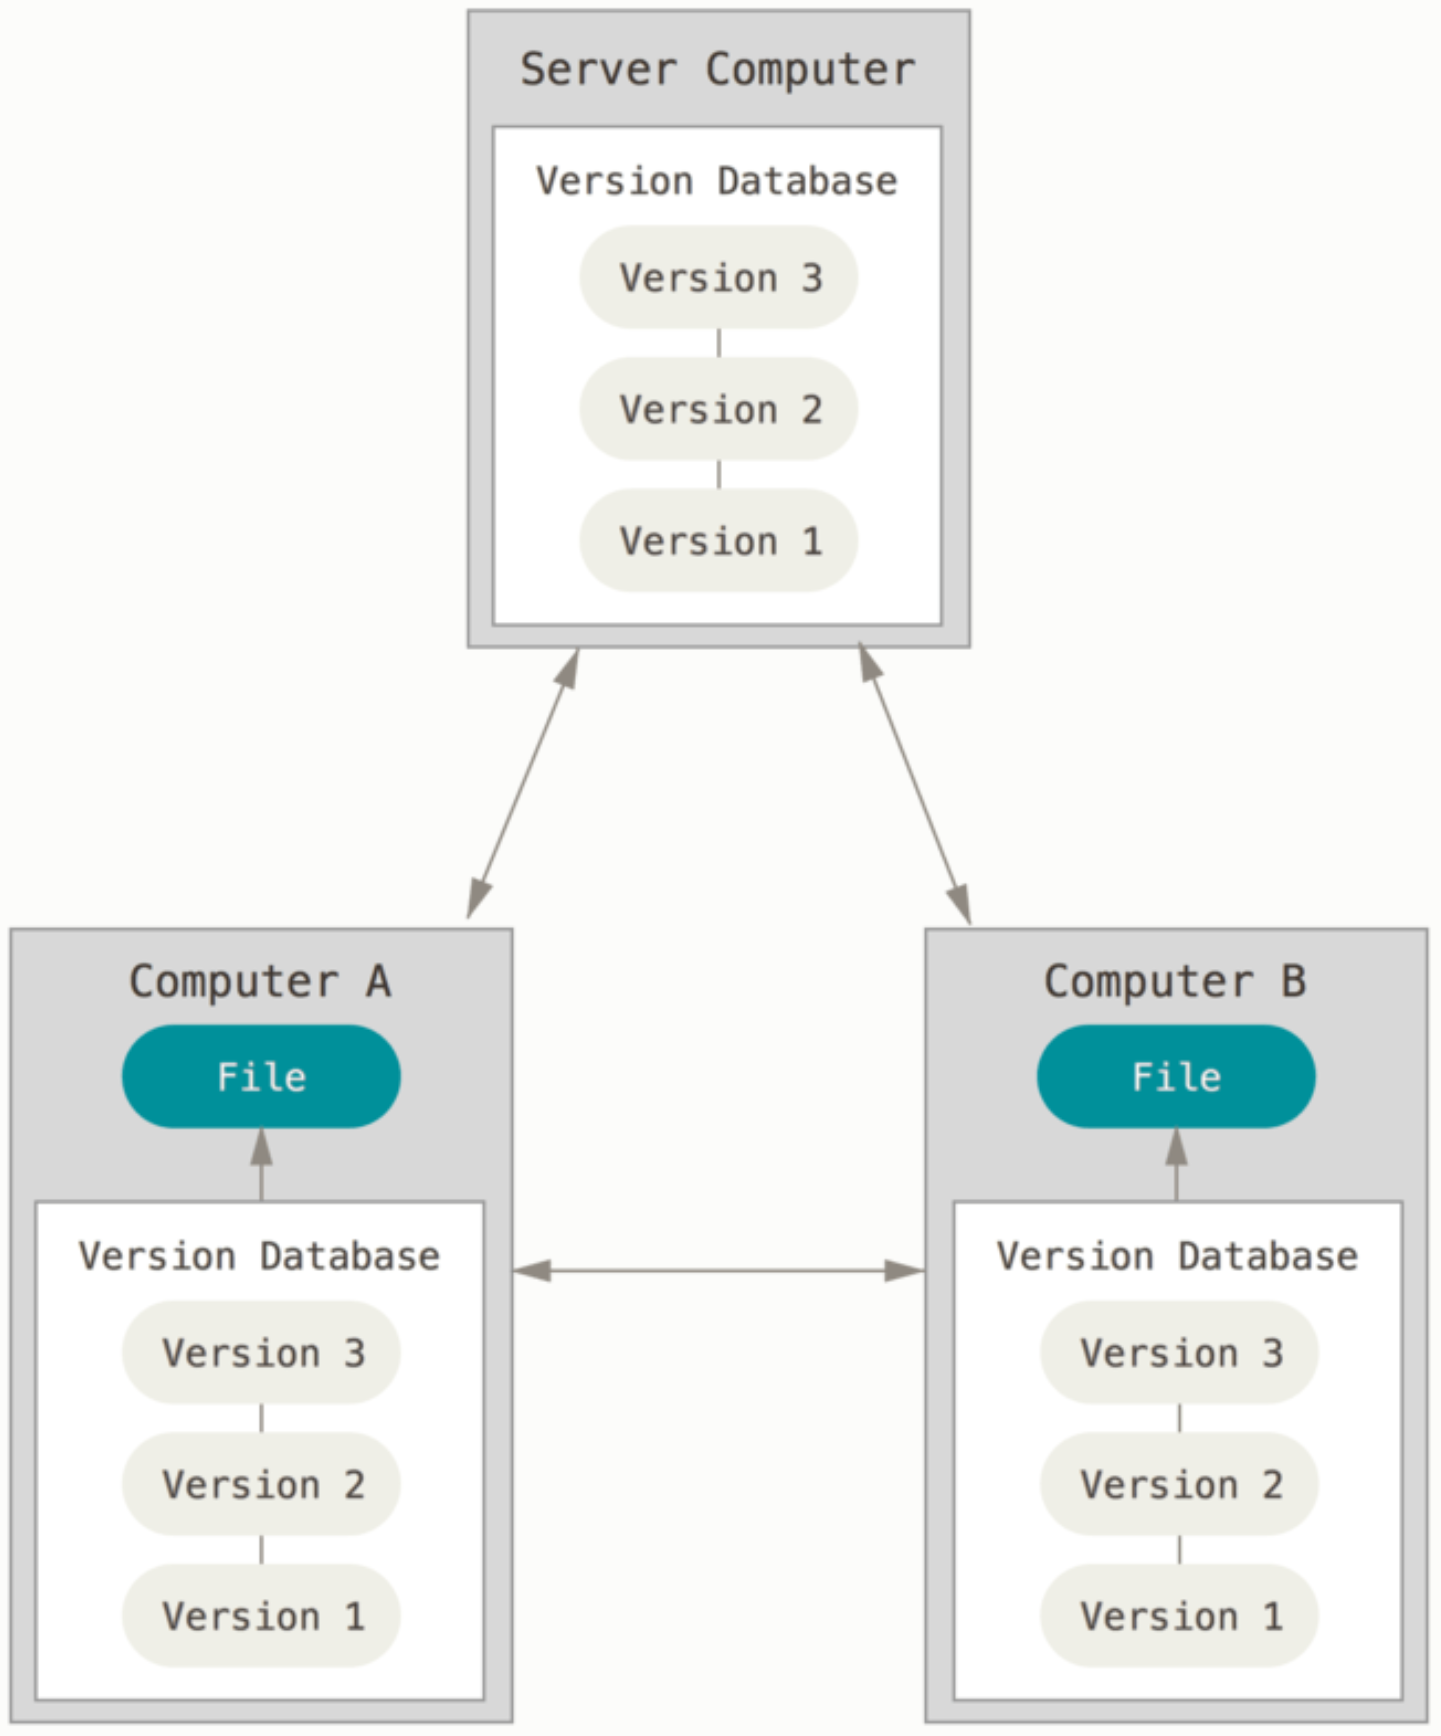
\includegraphics[width=0.6\textwidth]{distributedVcs.png}
	\attribution{https://git-scm.com/book/ru}
\end{center}

\section{Работа с Git}

Дальнейшее изложение является по сути кратким пересказом Git Book (\url{https://git-scm.com/book/en/v2}, или русская версия \url{https://git-scm.com/book/ru/v2}). Очень рекомендую оригинал, там написано кратко, по делу, с картинками и хорошим языком.

\subsection{Версионирование, дельты}

Так вот, Git на самом деле представляет из себя небольшую файловую систему с инструментами версионирования, работающими поверх неё. Git хранит ``снимки'' файловой системы рабочей папки на момент выполнения коммита, при этом изменённые файлы хранятся целиком, а неизменённые файлы в конкретном ``снимке'' вообще не хранятся --- Git просто делает для них ссылку на предыдущую версию. Это несколько отличается от того, как делал Subversion, который хранил дельты:

\begin{center}
	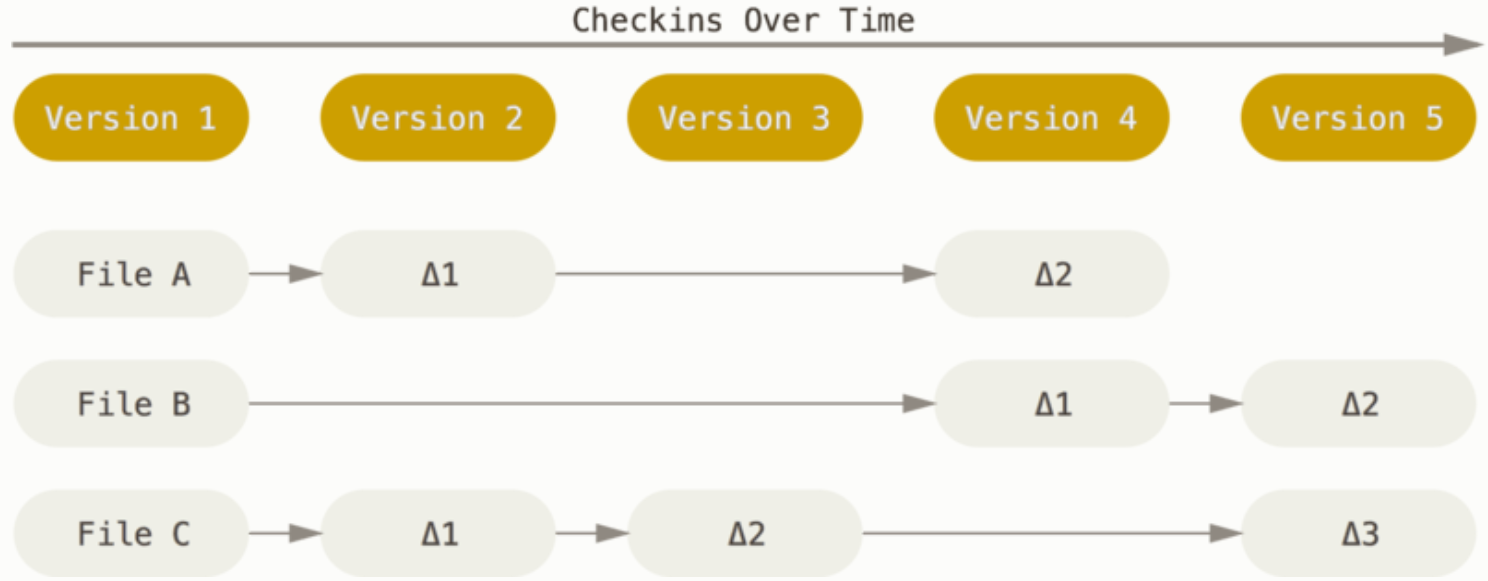
\includegraphics[width=0.7\textwidth]{deltaVersioning.png}
	\attribution{https://git-scm.com/book/ru}
\end{center}

Работа с версиями внутри Git выглядит скорее так:

\begin{center}
	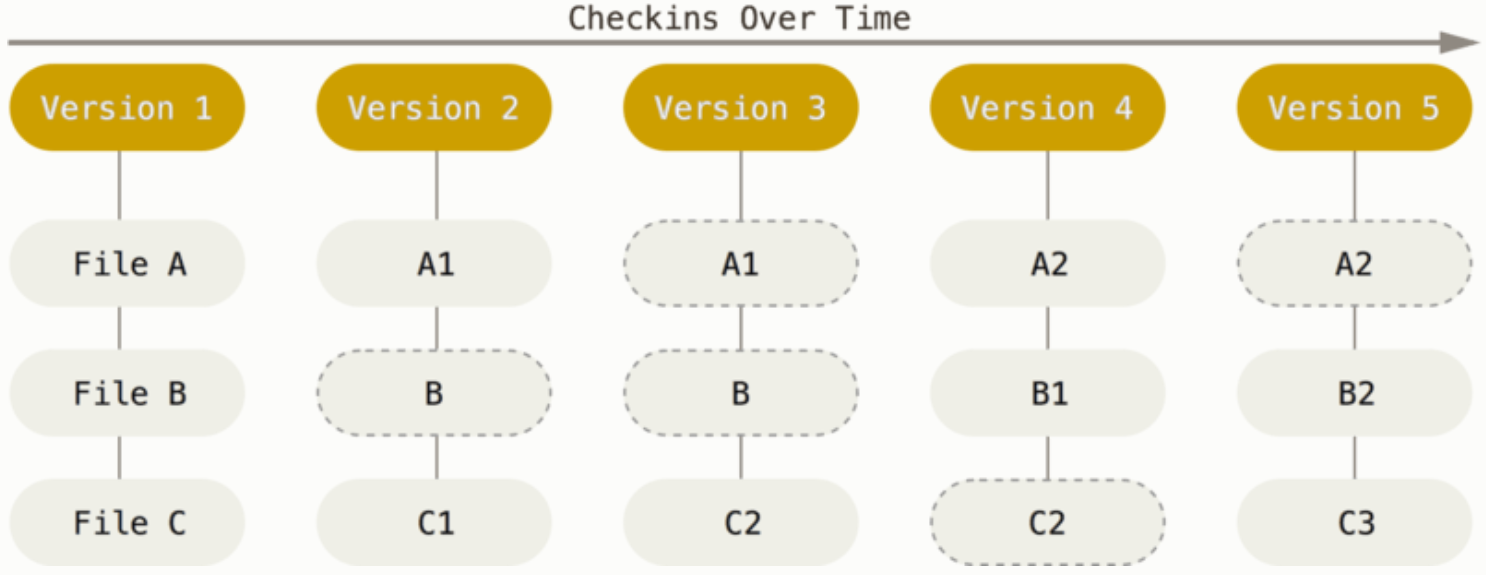
\includegraphics[width=0.7\textwidth]{snapshotVersioning.png}
	\attribution{https://git-scm.com/book/ru}
\end{center}

С точки зрения пользователя разницы особо нет, разве что репозиторий занимает больше места, зато работает быстрее. И так и так можно получить любую желаемую версию, либо взяв готовый снимок (за константное время), либо применив все дельты от первой версии (за линейное время). К тому же, все тулы для Git всё равно показывают дельты, когда речь идёт об изменениях. Например, вот так они выглядят на GitHub:

\begin{center}
	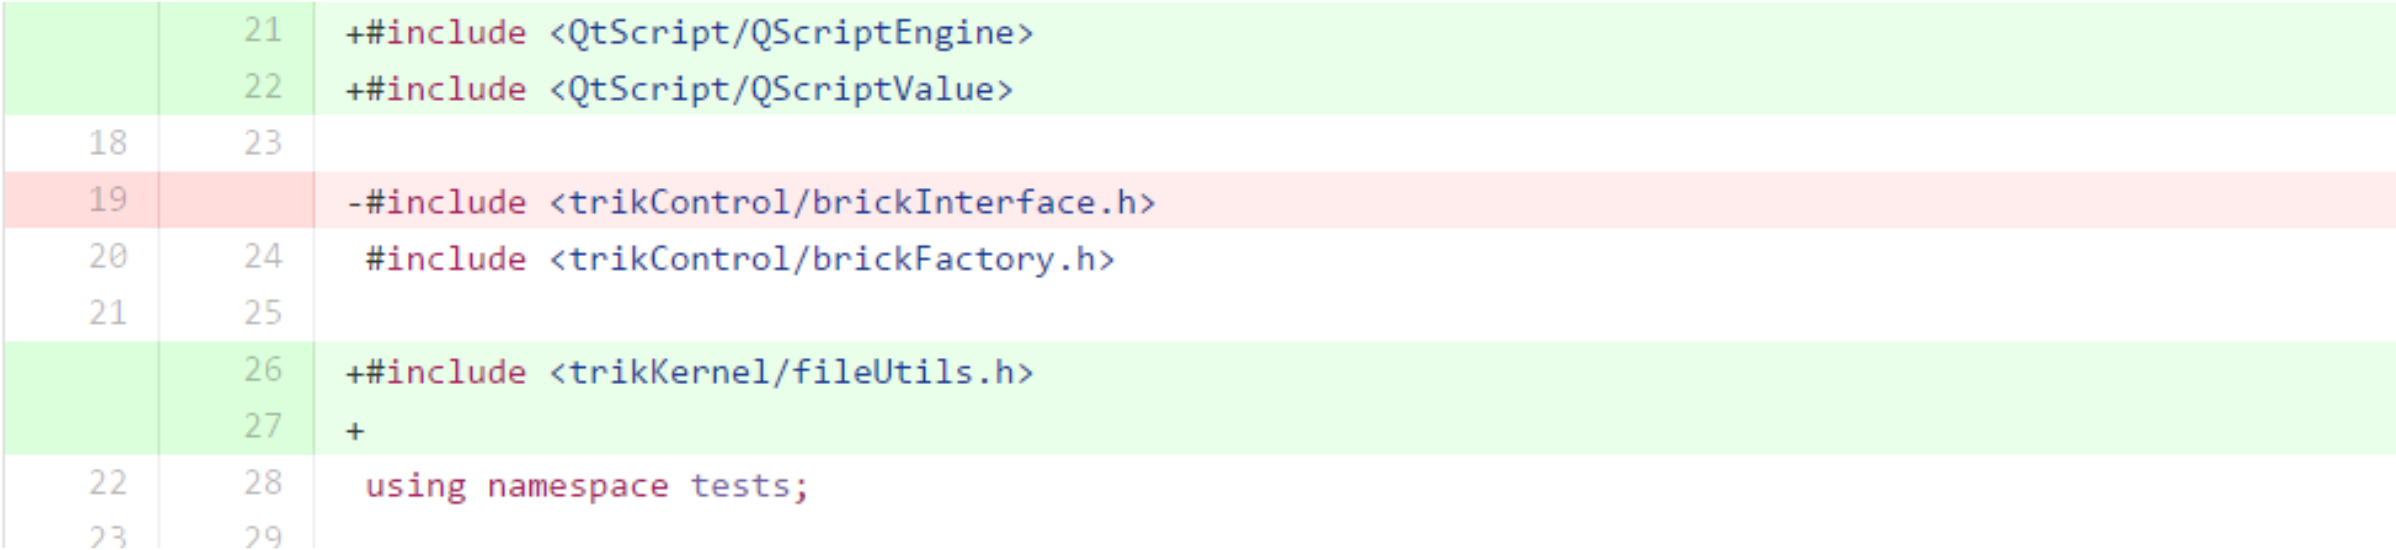
\includegraphics[width=0.9\textwidth]{delta.png}
\end{center}

\subsection{Жизненный цикл файла}

В Git каждый файл в вашем рабочем каталоге может находиться в одном из двух состояний: под версионным контролем (отслеживаемые) и нет (неотслеживаемые). Отслеживаемые файлы --- это те файлы, которые были в последнем слепке состояния проекта (snapshot); они могут быть неизмененными, измененными или подготовленными к коммиту/проиндексированными (staged). Неотслеживаемые файлы --- это всё остальное, любые файлы в вашем рабочем каталоге, которые не входили в ваш последний слепок состояния и не подготовлены к коммиту. Когда вы впервые клонируете репозиторий, все файлы будут отслеживаемыми и неизмененными, потому что вы только взяли их из хранилища (checked them out) и ничего пока не редактировали.

Как только вы отредактируете файлы, git будет рассматривать их как измененные, т.к. вы изменили их с момента последнего коммита. Вы индексируете (stage) эти изменения и затем фиксируете все индексированные изменения, а затем цикл повторяется:

\begin{center}
	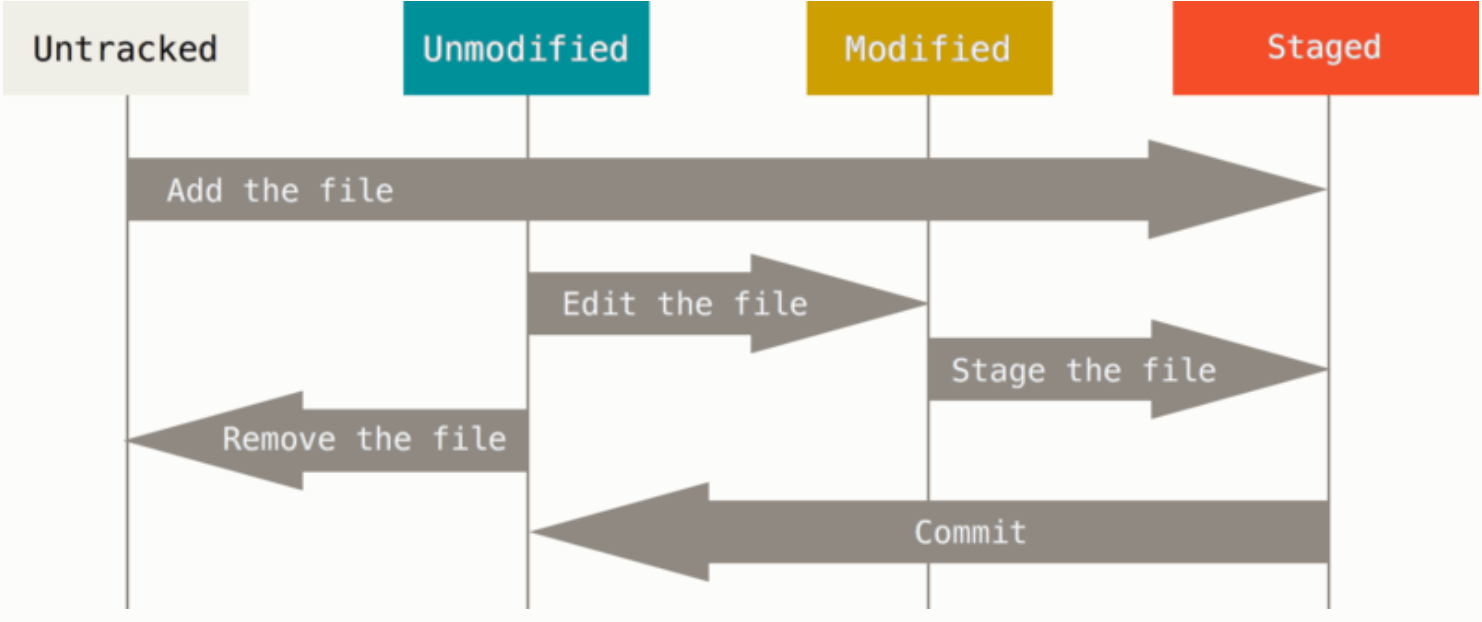
\includegraphics[width=0.75\textwidth]{fileLifeCycle.png}
\end{center}

\subsection{Основные команды}

Для того чтобы начать отслеживать (добавить под версионный контроль) новый файл, используется команда git add. Данная команда находит и подготавливает к фиксации (commit’у) сделанные в проекте или его части изменения (то есть её название ``добавить'' относится не к файлам, а к сделанным изменениям, которые добавляются в индекс для последующей фиксации/коммита). Это важная особенность Git, потому что Subversion, например, оперирует файлами целиком. В Git же возможно часть изменений внутри одного файла закоммитить, а часть оставить на будущее.

Команда git status позволяет узнать, какие файлы в каком состоянии находятся. Для того, чтобы узнать, что конкретно поменялось, а не только какие файлы были изменены --- вы можете использовать команду git diff. Вы, скорее всего, будете использовать эти команды для получения ответов на два вопроса: что вы изменили, но еще не проиндексировали, и что вы проиндексировали и собираетесь коммитить. Если git status отвечает на эти вопросы слишком обобщенно, то git diff показывает вам непосредственно добавленные и удаленные строки --- собственно патч (patch). Важно отметить, что git diff сама по себе не показывает все изменения сделанные с последнего коммита --- только те, что еще не проиндексированы. Такое поведение может сбивать с толку, так как если вы проиндексируете все свои изменения, то git diff ничего не вернет.

Чтобы сделать коммит (фиксацию изменений), нужно выполнить команду git commit. Эта команда откроет выбранный вами текстовый редактор, в котором нужно будет написать комментарий к данному коммиту. При использовании графических утилит типа TortoiseGit у вас откроется специальное окошко для ввода комментария. Комментарии должны быть осмысленными, потому что это единственный способ быстро понять, что было сделано в том или ином коммите. Т.е. если вы разрабатываете большую систему и хотите найти какой-то давний коммит, то это будет гораздо проще сделать просмотром лога коммитов с комментариями, чем диффов. Таким образом, у нас коммиты с пустым или неадекватным текстом в комменте будут страшно караться. В комменте не нужно писать, какие файлы поменялись (это и так видно по диффу), пишите, почему они поменялись --- что вы такого сделали, как изменилась логика, что добавилось/удалилось и т.п.

Довольно типична ситуация, когда хочется поправить последний коммит (например, забыли добавить какие-то файлы или написали плохой комментарий). Это можно сделать, выполнив commit с опцией --amend:

\begin{minted}{text}
$ git commit --amend
\end{minted}

Эта команда берёт индекс и использует его для коммита. Если после последнего коммита не было никаких изменений (например, вы запустили приведённую команду сразу после предыдущего коммита), то состояние проекта будет абсолютно таким же и всё, что вы измените --- это комментарий к коммиту. Появится всё тот же редактор для комментариев к коммитам, но уже с введённым комментарем к последнему коммиту. Вы можете отредактировать это сообщение так же как обычно, и оно перепишет предыдущее.

Кстати, комментарий удобнее вводить прямо из командной строки, ключом -m:

\begin{minted}{text}
$ git commit -m"Some useful comment"
\end{minted}

Для того чтобы удалить файл из git, вам необходимо удалить его из отслеживаемых файлов (точнее, удалить его из вашего индекса) а затем выполнить коммит. Это позволяет сделать команда git rm, которая также удаляет файл из вашего рабочего каталога, так что вы в следующий раз не увидите его как неотслеживаемый.

Историю коммитов позволяет увидеть команда git log. У нее есть много всяких параметров, которые позволяют красиво форматировать вывод истории. Например, можно сделать алиас на команду 

\begin{minted}{text}
git log --pretty=format:\"%h %ad | %s%d [%an]\" --graph --date=short
\end{minted}

который удобным образом показывает хэш и дерево коммитов, дату, комментарий и автора коммита. Всякие TortoiseGit позволяют рисовать красивые картинки. На GitHub тоже есть рисовалка дерева коммитов.

Чтобы откатить локальные непроиндексированные изменения (поправили файл и поняли, что лучше бы этого не делать и вернуть как было), нужно выполнить команду git checkout [имяфайла].

\subsection{Работа с удалёнными репозиторями}

Для совместной разработки с git настраивают один или несколько удалённых репозиториев (как правило, в каком-нибудь облачном сервисе типа GitHub или BitBucket, но часто корпоративная политика безопасности заставляет настроить репозиторий в локалке). Совместная работа включает в себя управление удалёнными репозиториями и помещение/push и получение/pull данных в и из них тогда, когда нужно обменяться результатами работы. Управление удалёнными репозиториями включает умение добавлять удалённые репозитории, удалять те из них, которые больше не действуют, умение управлять различными удалёнными ветками и определять их как ослеживаемые (tracked) или нет и прочее. 

Чтобы просмотреть какие удалённые репозитории знает ваш локальный репозиторий, следует выполнить команду git remote. Она перечисляет список имён-сокращений для всех уже указанных удалённых репозиториев (по сути, remote --- это просто имя для URL, по которому можно найти репозиторий). Если вы склонировали ваш репозиторий, у вас должен отобразиться по крайней мере origin --- это имя по умолчанию, которое git присваивает серверу, с которого вы этот репозиторий склонировали.

Когда ваш проект достигает момента, когда вы хотите поделиться своими наработками, вам необходимо отправить (push) их в главный репозиторий. Команда для этого действия простая: git push [удаленный\_сервер] [ветка]. Чтобы отправить вашу ветку master на сервер origin (клонирование настраивает оба этих имени автоматически), вы можете выполнить следующую команду для отправки наработок обратно на сервер:

\begin{minted}{text}
$ git push origin master
\end{minted}

Или просто

\begin{minted}{text}
$ git push
\end{minted}

Выкладывание новой ветки несколько хитрее:

\begin{minted}{text}
$ git push -u origin [локальное имя ветки]:[удалённое имя ветки]
\end{minted}

Ключ -u говорит, что теперь эта ветка в вашем репозитории следит (tracking) за веткой удалённого репозитория и последующие команды push/pull будут получать изменения из правильной удалённой ветки.

Вообще, push срабатывает только в случае, если вы клонировали с сервера, на котором у вас есть права на запись, и если никто другой с тех пор не выполнял команду push. Если вы и кто-то ещё одновременно клонируете, затем он выполняет команду push, а затем команду push выполняете вы, то ваш push точно будет отклонён. Вам придётся сначала запуллить (pull) их изменения и смерджить с вашими. Только после этого вам будет позволено выполнить push.

Для получения изменений из удалённых репозиториев следует выполнить git fetch [remote-name]. Данная команда связывается с указанным удалённым репозиторием и забирает все те коммиты, которых у вас ещё нет. После того как вы выполнили команду, у вас должны появиться ссылки на все ветки из этого репозитория. В частности, теперь эти ветки в любой момент могут быть просмотрены или слиты.

Когда вы клонируете репозиторий, команда clone автоматически добавляет этот удалённый репозиторий под именем origin. Таким образом git fetch origin извлекает все наработки, отправленные (push) на этот сервер после того, как вы склонировали его (или получили изменения с помощью fetch). Важно отметить, что команда fetch забирает данные в ваш локальный репозиторий, но не сливает их с какими-либо вашими наработками, и не модифицирует то, над чем вы работаете в данный момент. Вам необходимо вручную слить эти данные с вашими, когда вы будете готовы.

Если у вас есть ветка, настроенная на отслеживание удалённой ветки, то вы можете использовать команду git pull. Она автоматичеси извлекает и затем сливает данные из удалённой ветки в вашу текущую ветку. Обычно так все и делают вместо git fetch + git merge, но pull получает только коммиты из одной ветки, в отличие от fetch, которая получает всё. К тому же по умолчанию команда git clone автоматически настраивает вашу локальную ветку master на отслеживание удалённой ветки master на сервере, с которого вы клонировали (подразумевается, что на удалённом сервере есть ветка master). Выполнение git pull как правило извлекает (fetch) данные с сервера, с которого вы изначально склонировали, и автоматически пытается слить (merge) их с кодом, над которым вы в данный момент работаете.

\subsection{Что такое на самом деле коммиты и ветки}

Теперь несколько больше технических подробностей. Когда мы исполняем, например, такую команду:

\begin{minted}{text}
$ git add README test.rb LICENSE
$ git commit -m 'initial commit of my project'
\end{minted}

на самом деле создаётся так называемый commit object (на деле --- просто файл), хранящий метаинформацию о коммите и ссылку на объект tree object, который хранит информацию о файлах, которые поменялись в этом коммите. tree object, в свою очередь, хранит ссылку на объект типа blob, который уже хранит в себе содержимое файла. Все эти штуки --- это просто файлы, ссылки --- это просто имена файлов. Имена, правда, не такие, как были в рабочей копии, а SHA-1-хеши их содержимого.

Выглядит это примерно вот так:

\begin{center}
	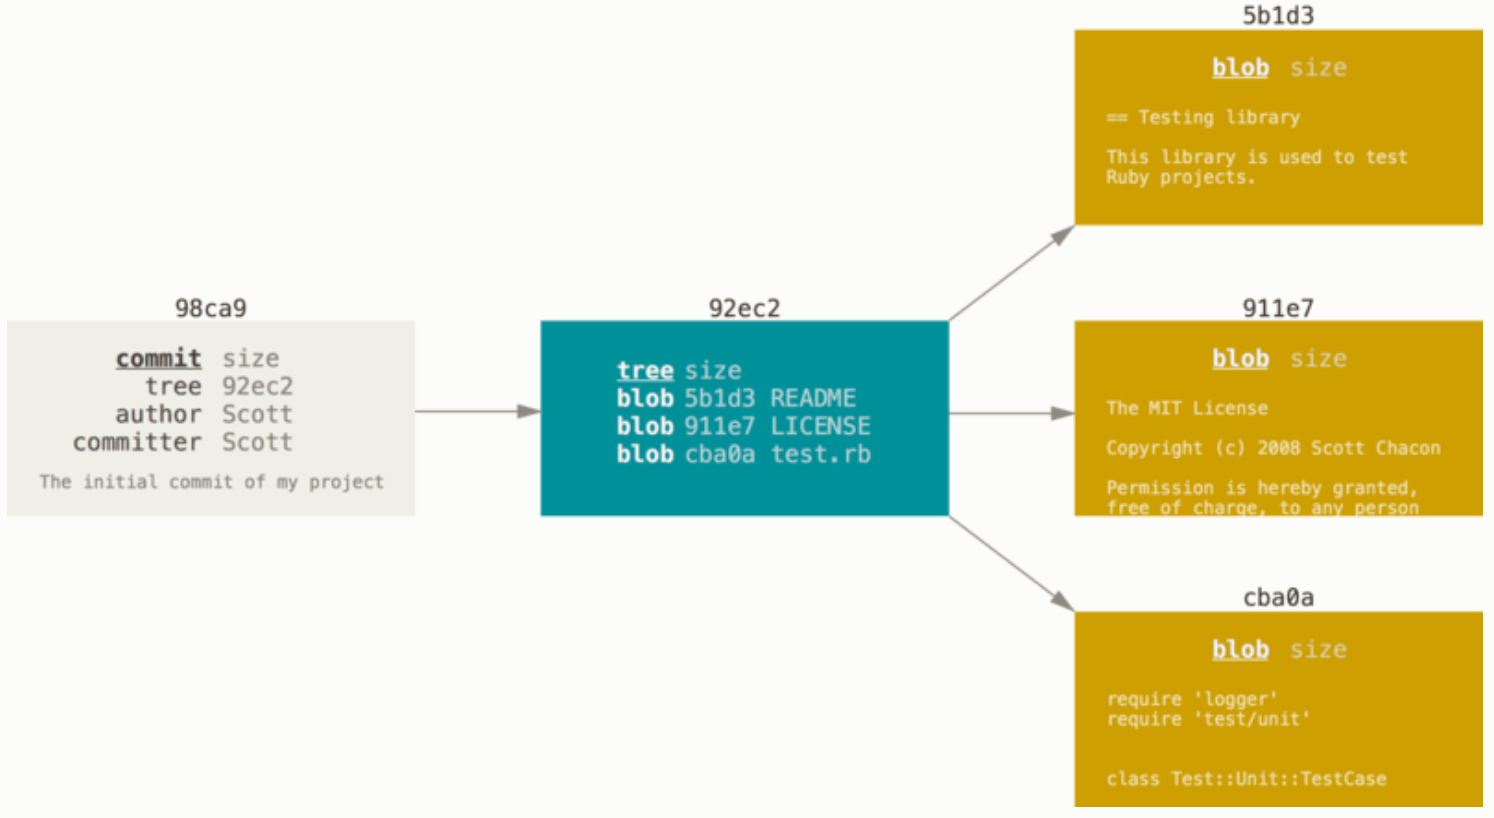
\includegraphics[width=0.85\textwidth]{blobs.png}
	\attribution{https://git-scm.com/book/ru}
\end{center}

Да, на самом деле Git --- это хеш-таблица, отображающая SHA-1-хеш файла в его содержимое. А поскольку все объекты в Git хранятся как файлы, то хеш имеет ключевое значение --- он фактически работает как указатель.

Собственно, даёт возможность выстраивать историю версий то, что каждый commit object ссылается на предыдущий commit object, на базе которого он был создан:

\begin{center}
	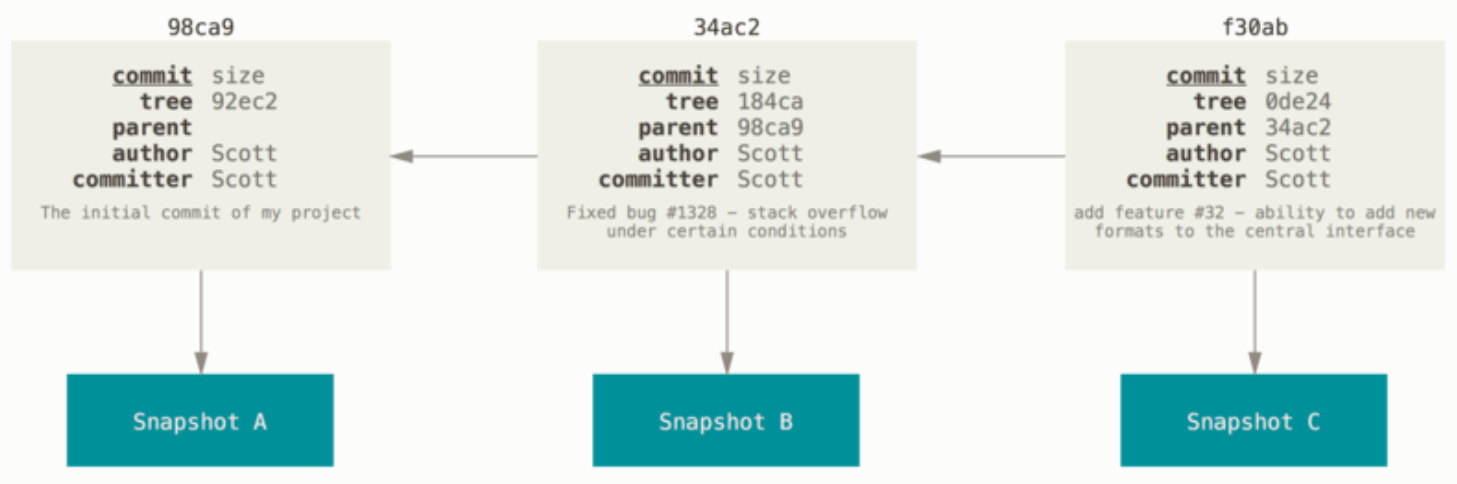
\includegraphics[width=0.85\textwidth]{commits.png}
	\attribution{https://git-scm.com/book/ru}
\end{center}

В принципе, мы уже можем собрать дерево коммитов, но пользоваться им будет неудобно, потому что надо будет помнить SHA-1-хеши конкретных коммитов, чтобы между ними переключаться. На помощь приходят ветки, которые на самом деле просто именованные указатели на коммит:

\begin{center}
	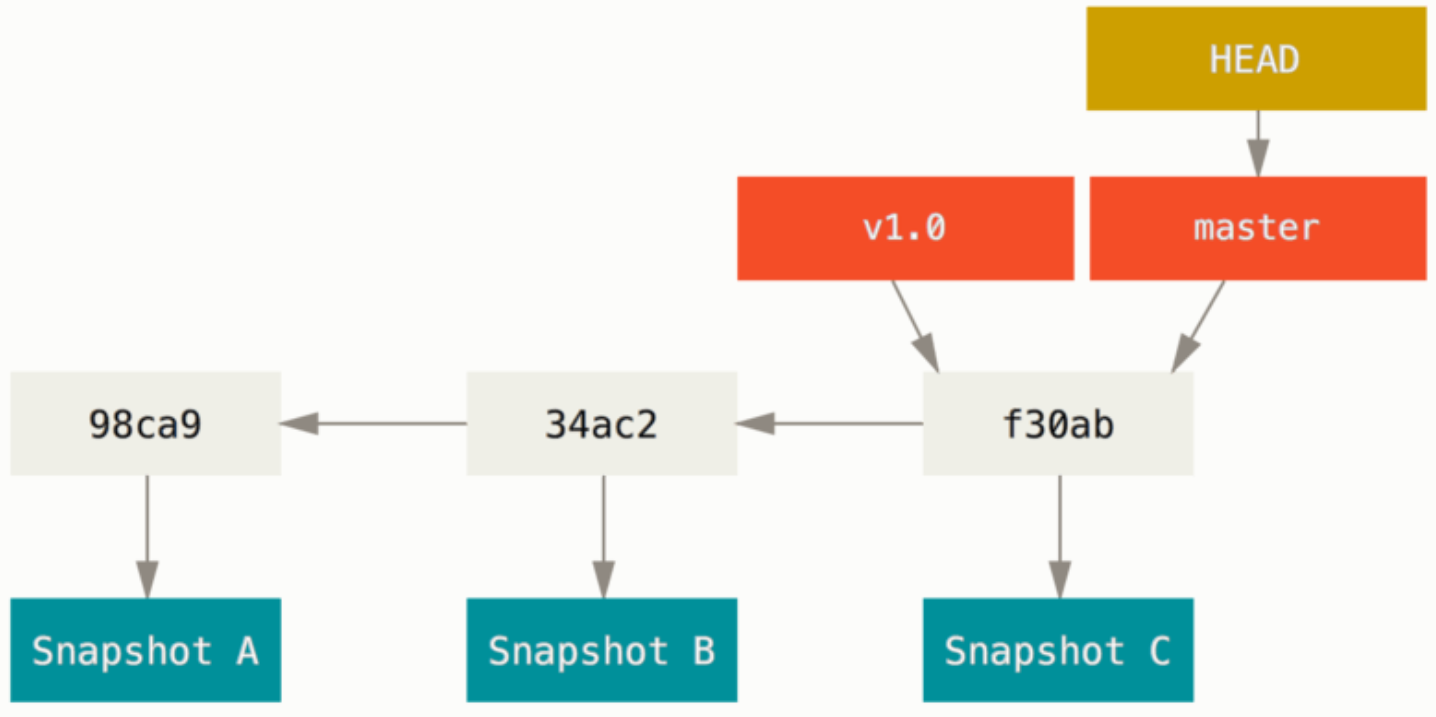
\includegraphics[width=0.8\textwidth]{branches.png}
	\attribution{https://git-scm.com/book/ru}
\end{center}

Ветки на самом деле --- это частный случай ссылок (Reference), помимо веток бывают ещё тэги и символические ссылки. И ветки --- это, как и обычно, отдельные файлы, которые тоже хранятся в репозитории, но, в отличие от большинства остальных файлов, называются они по-человечески. Вот как выглядит структура файлов со всем вышеизложенным:

\begin{center}
	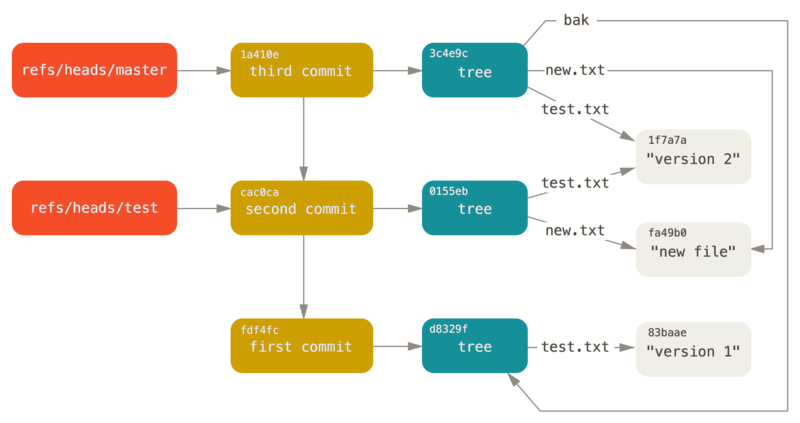
\includegraphics[width=0.9\textwidth]{gitRefs.png}
	\attribution{https://git-scm.com/book/ru}
\end{center}

Имея ветки, можно не учить наизусть хеши коммитов, но среди веток должна быть одна, с которой мы сейчас работаем, и механизм переключения веток. Это обеспечивается символической ссылкой HEAD, которая всегда хранит ссылку на ветку, исходники из которой сейчас находятся в рабочей папке:

\begin{minted}{text}
$ cat .git/HEAD
ref: refs/heads/master
\end{minted}

При создании ветки происходит не более чем создание нового указателя на тот коммит, на который сейчас указывает ветка, на которую указывает HEAD, как бы запутанно это ни звучало:

\begin{minted}{text}
$ git branch testing
\end{minted}

\begin{center}
	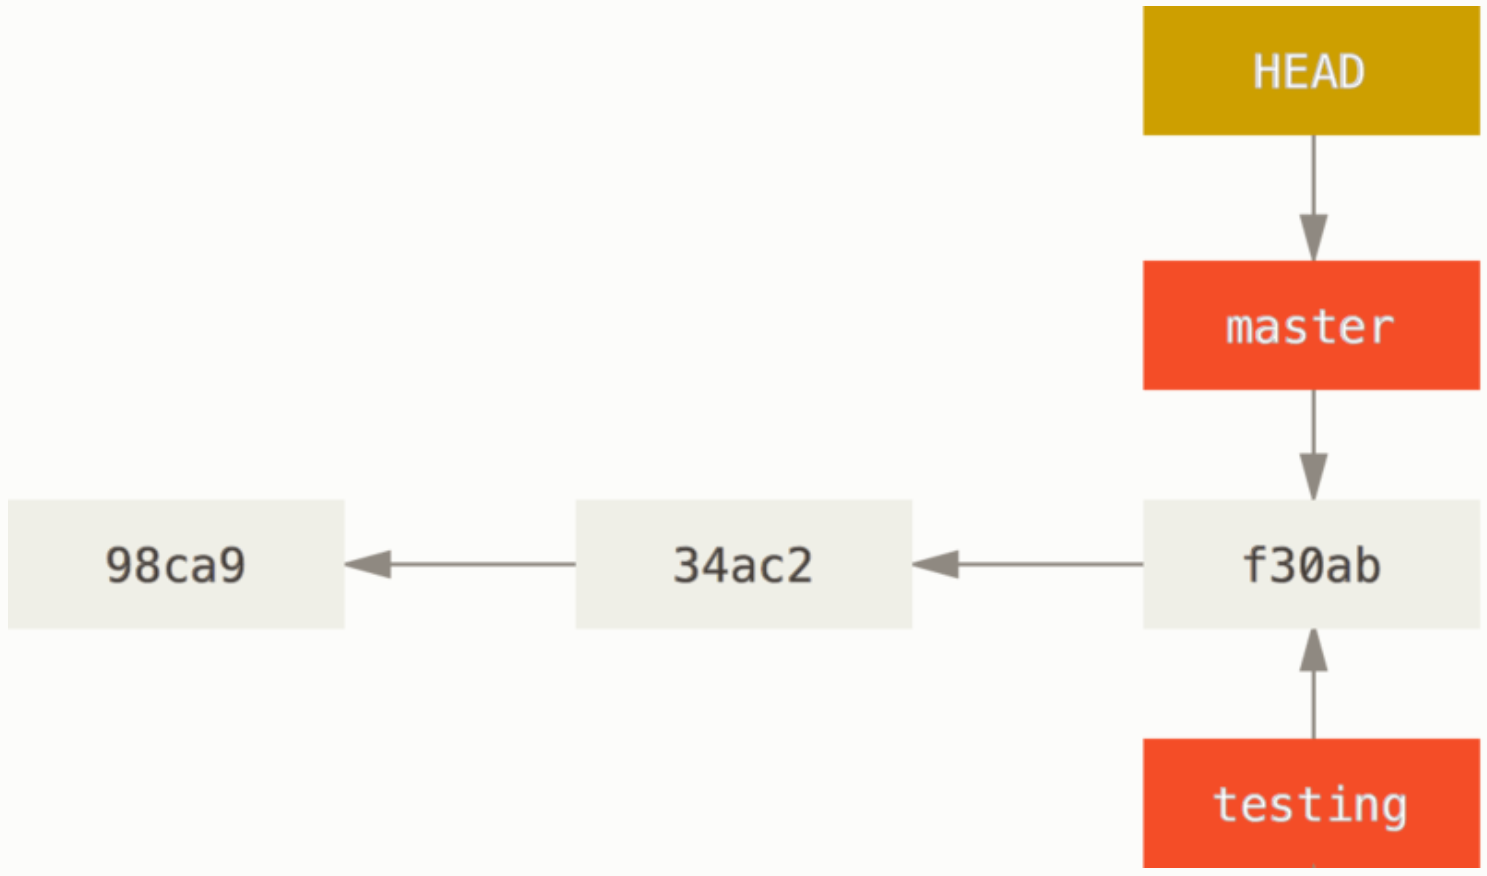
\includegraphics[width=0.7\textwidth]{creatingBranch.png}
	\attribution{https://git-scm.com/book/ru}
\end{center}

Переключение ветки --- это несколько более сложный процесс. Во-первых, Git копирует из репозитория файлы, относящиеся к ветке, на которую мы переключаемся, в рабочую папку, и удаляет файлы, которые находятся под управлением системы контроля версий, но к нужной ветке не относятся. Во-вторых, при этом Git проверяет, что эти манипуляции не приведут к потере данных --- удалению незакоммиченного файла или перетиранию изменённого файла. В-третьих, HEAD переставляется на новую ветку:

\begin{minted}{text}
$ git checkout testing
\end{minted}

\begin{center}
	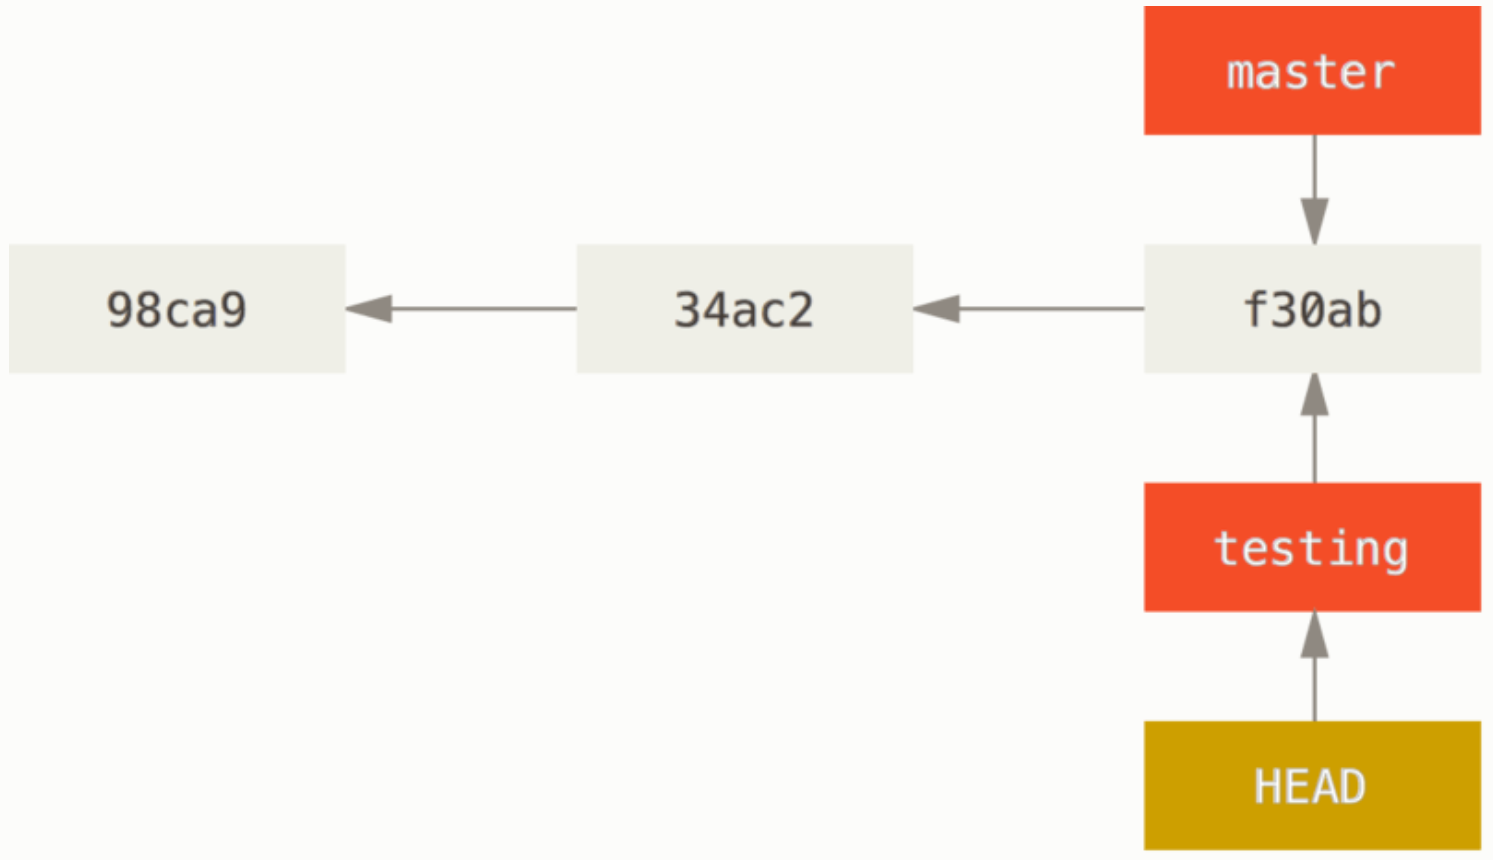
\includegraphics[width=0.7\textwidth]{checkout.png}
	\attribution{https://git-scm.com/book/ru}
\end{center}

Коммит --- это создание нового Commit Object-а (с созданием соответствующих ему Tree Object-а и Blob-ов), выставление ему родителем текущего коммита, на который указывает HEAD, и продвижение ветки, на который указывает HEAD:

\begin{minted}{text}
<Что-то поделали с файлами в рабочей копии>
$ git add <изменения, которые хотим коммитить>
$ git commit -m 'made a change'
\end{minted}

\begin{center}
	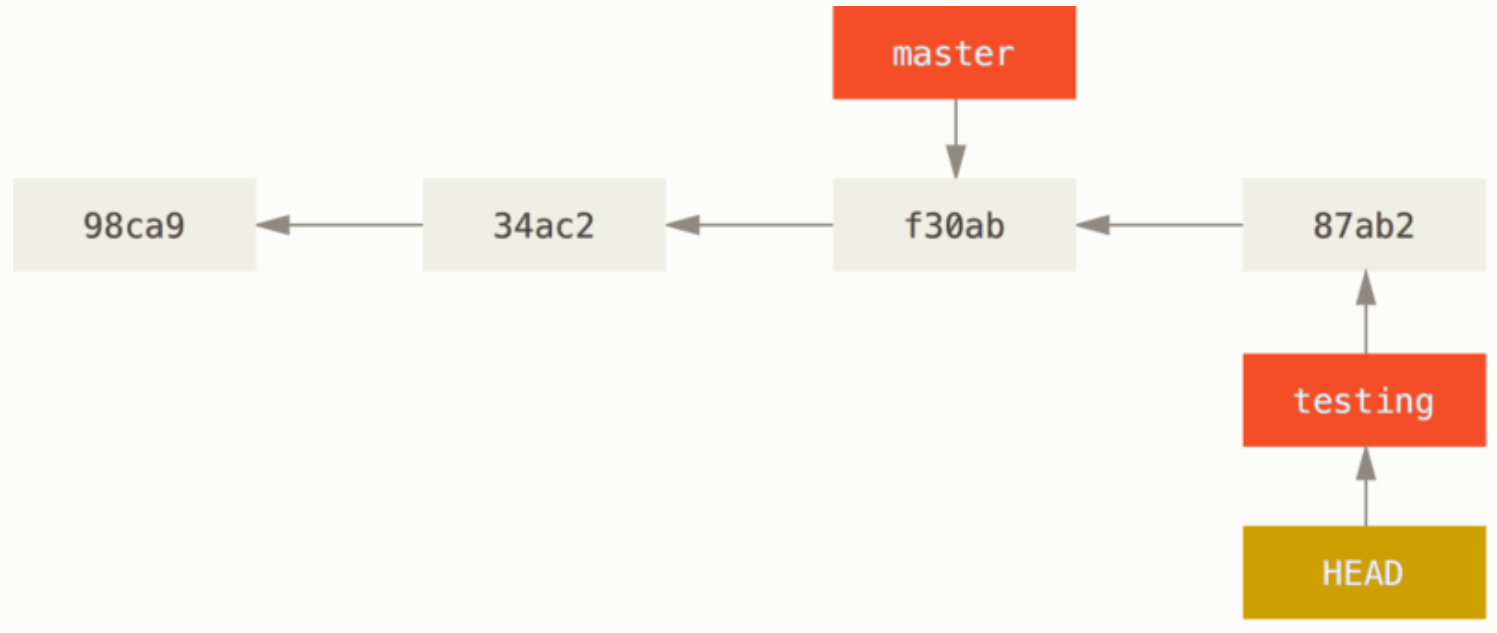
\includegraphics[width=0.8\textwidth]{newCommit.png}
	\attribution{https://git-scm.com/book/ru}
\end{center}

Теперь, положим, мы захотели переключиться обратно на master:

\begin{minted}{text}
$ git checkout master
\end{minted}

\begin{center}
	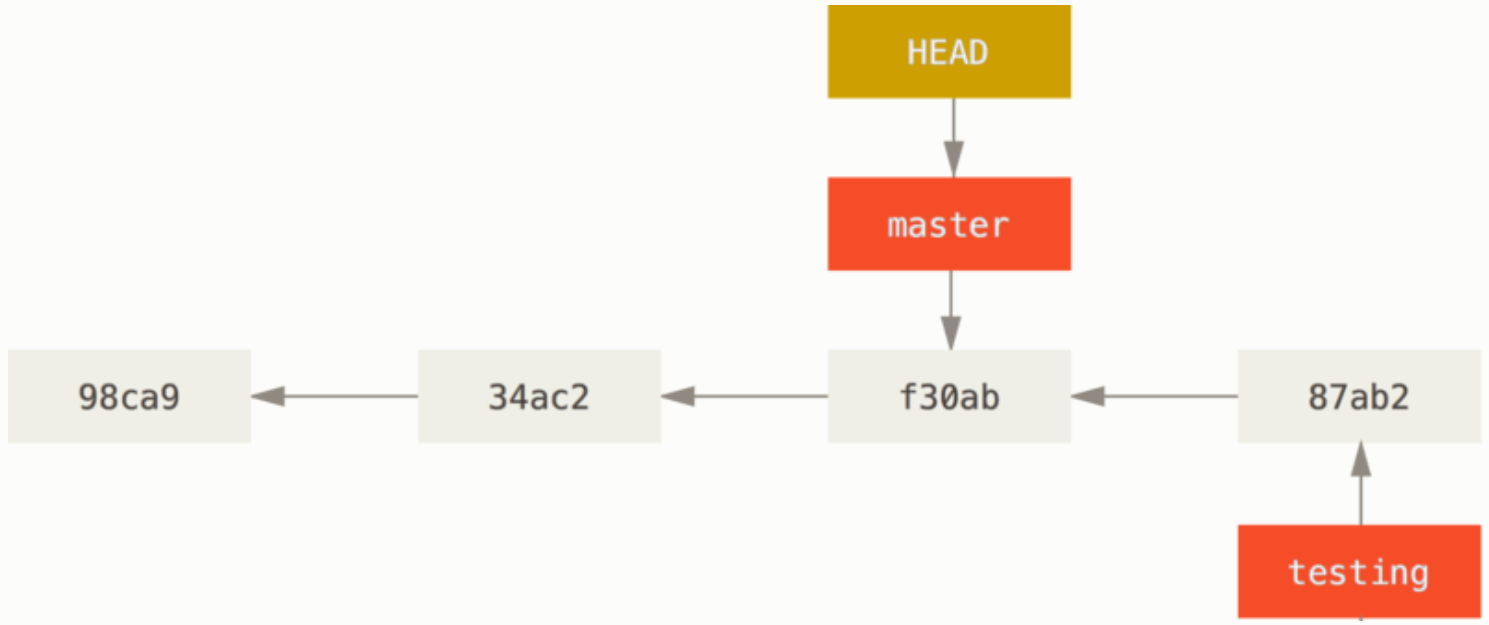
\includegraphics[width=0.8\textwidth]{checkoutToMaster.png}
	\attribution{https://git-scm.com/book/ru}
\end{center}

Делаем коммит там:

\begin{minted}{text}
<Что-то поделали с файлами в рабочей копии>
$ git add <изменения, которые хотим коммитить>
$ git commit -m 'made other changes'
\end{minted}

\begin{center}
	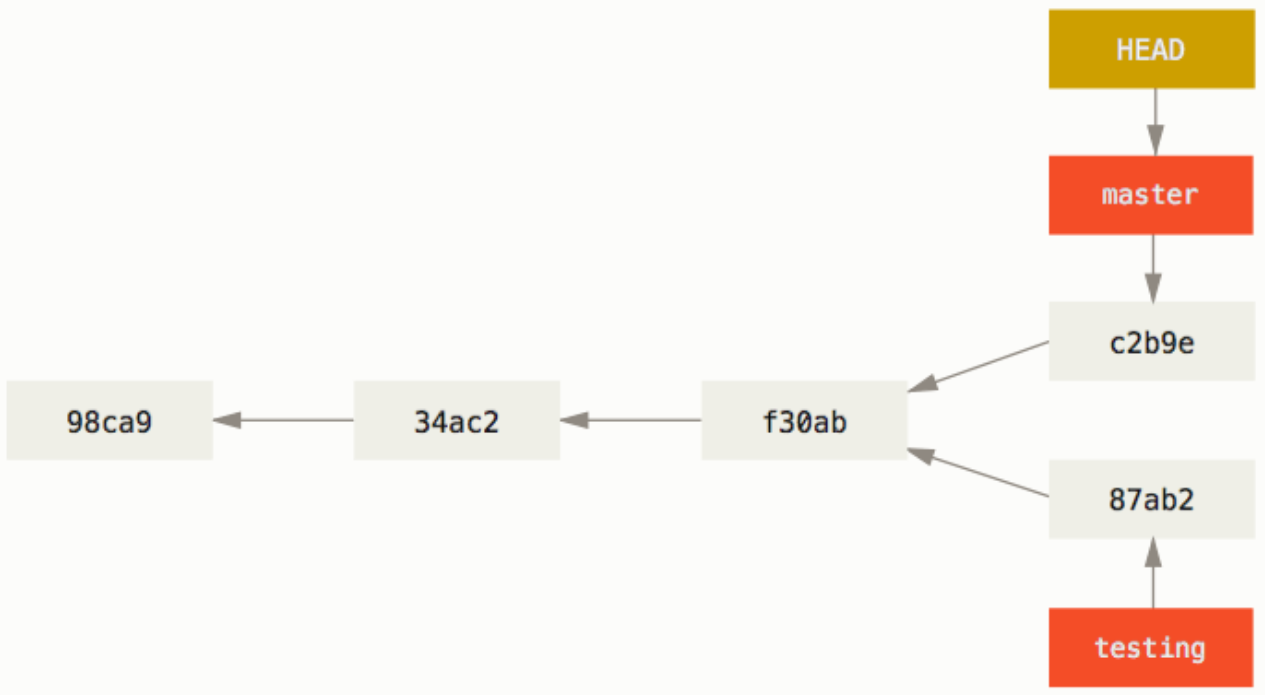
\includegraphics[width=0.8\textwidth]{newCommitToMaster.png}
	\attribution{https://git-scm.com/book/ru}
\end{center}

\subsection{Слияние веток}

Теперь у нас получились две разные ветки работы, имеющие общего предка, так что можно выполнить слияние. Допустим, мы хотим слить изменения из testing в master:

\begin{minted}{text}
$ git checkout master
Switched to branch 'master'
$ git merge testing
Merge made by the 'recursive' strategy.
index.html |    1 +
1 file changed, 1 insertion(+)
\end{minted}

\begin{center}
	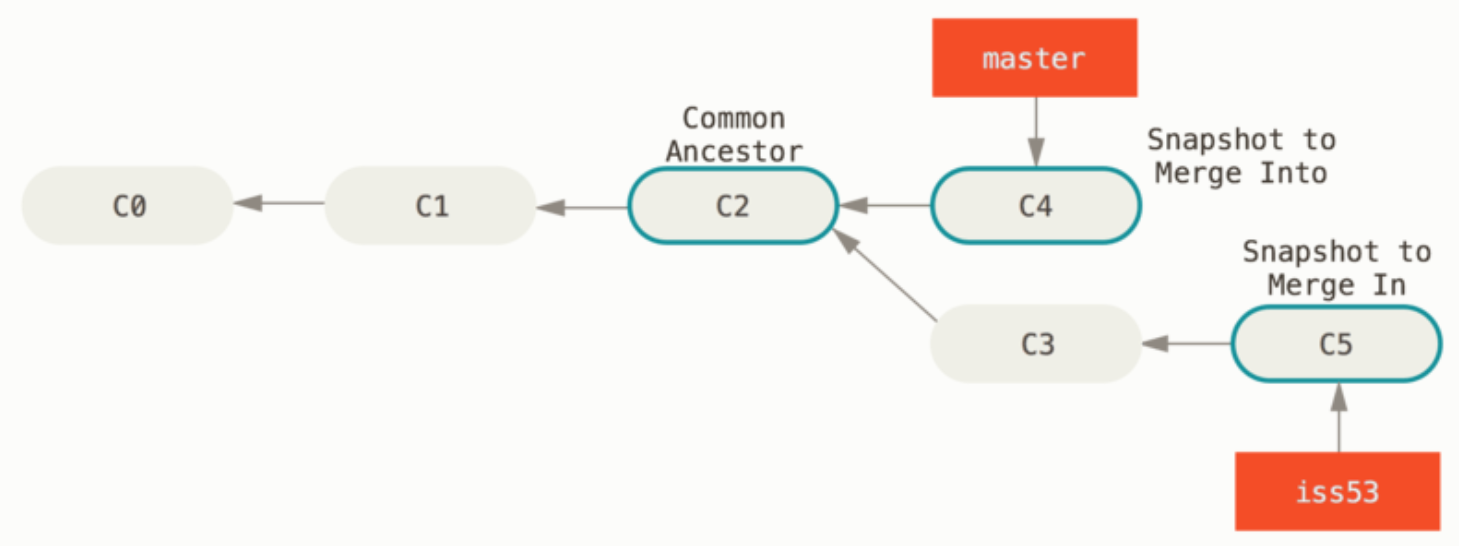
\includegraphics[width=0.8\textwidth]{merge.png}
	\attribution{https://git-scm.com/book/ru}
\end{center}

При этом создаётся так называемый merge commit и, если нет конфликтов, все изменения из ветки применяются к master-у. Концептуально это можно воспринимать так, что Git считает дифф между файлами из двух веток и применяет этот дифф. Merge commit Git обрабатывает особо --- у него два родителя, Git знает, что это merge commit, и, например, GitHub не учитывает такие коммиты в разных статистиках. Получается как-то так:

\begin{center}
	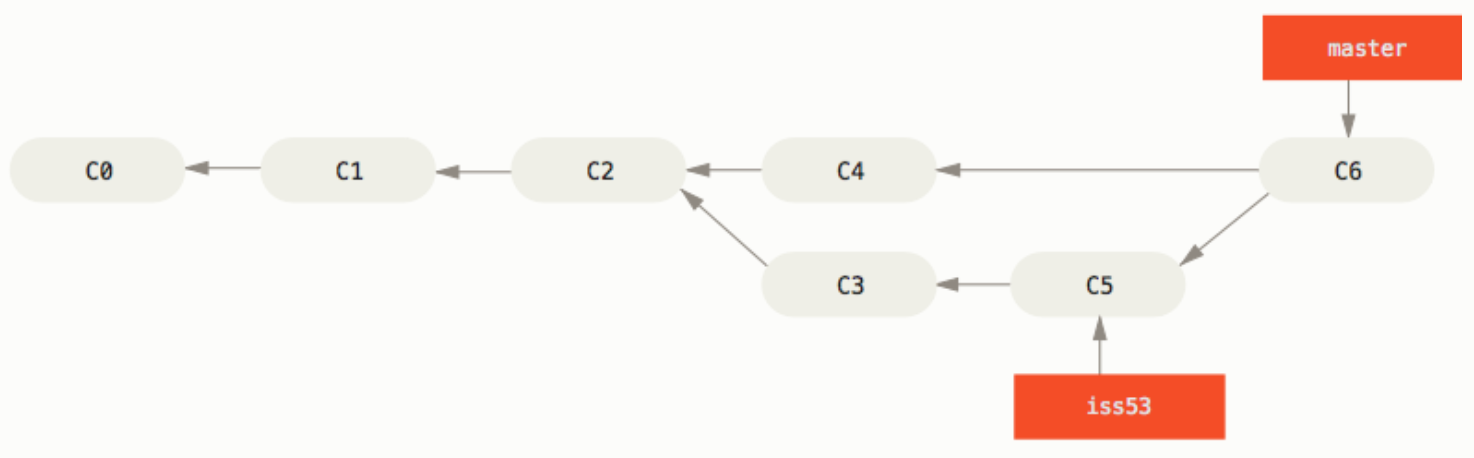
\includegraphics[width=0.8\textwidth]{mergeResult.png}
	\attribution{https://git-scm.com/book/ru}
\end{center}

Естественно, в реальной разработке чистый мердж --- это большая редкость. Чаще всего имеются конфликты --- когда изменения в обоих ветках затрагивают одно и то же место. Обратите внимание, что если даже изменения в двух ветках были в одном файле, но в разных его местах, Git смерджит такой файл самостоятельно и конфликта не возникнет, проблема возникает только в том случае, когда Git реально сам не может решить, что делать --- то ли в одной из веток код свежее и надо взять его, то ли надо взять оба варианта и расположить первый под вторым или второй под первым. В таком случае решение предлагается принять разработчику. Создаётся временная ссылка MERGE\_HEAD, указывающая на ветку, из которой мы мерджим изменения, и для каждого файла с конфликтом создаётся ещё два файла --- как было в HEAD, как было в MERGE\_HEAD, и как теперь. ``Как теперь'' содержит маркеры \mintinline{text}|<<< === >>>|, обозначающие места с конфликтами, специально, чтобы код не скомпилился:

\begin{center}
	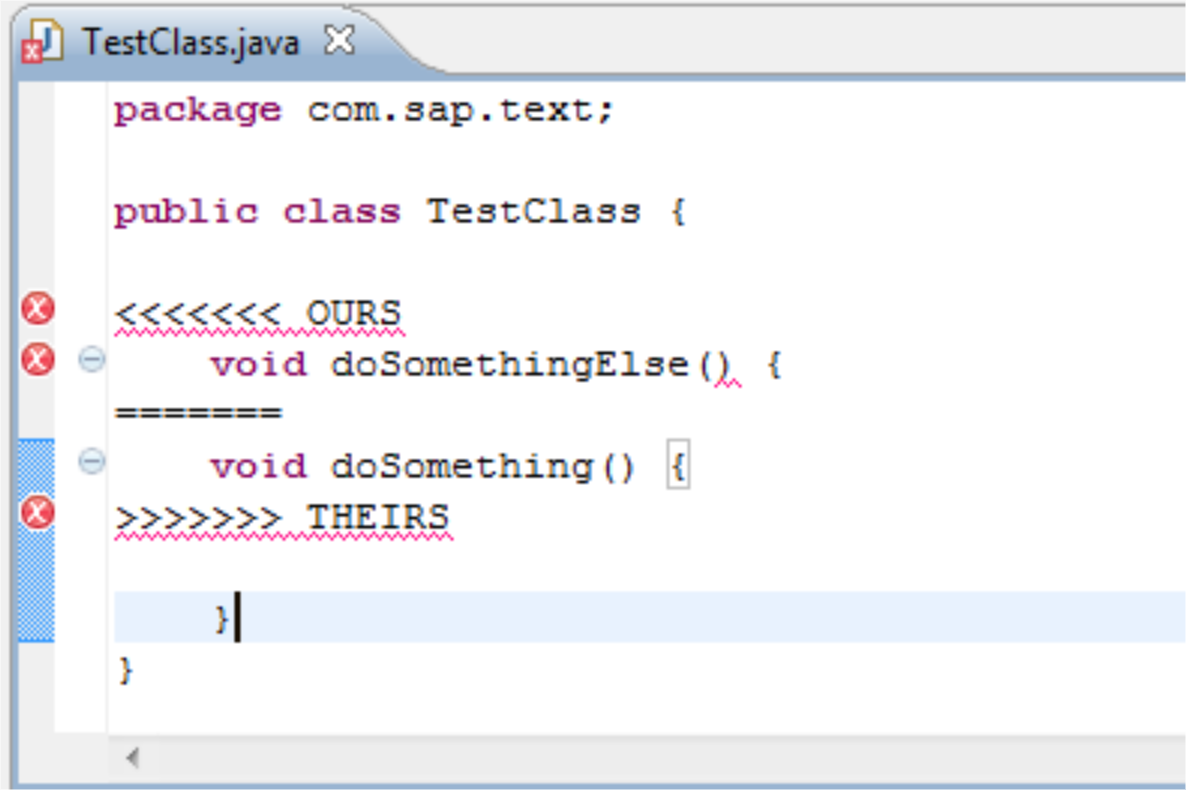
\includegraphics[width=0.5\textwidth]{conflictsInCode.png}
\end{center}

Хорошая новость в том, что большинство графически инструментов умеют показывать и редактировать конфликты красиво и удобно:

\begin{center}
	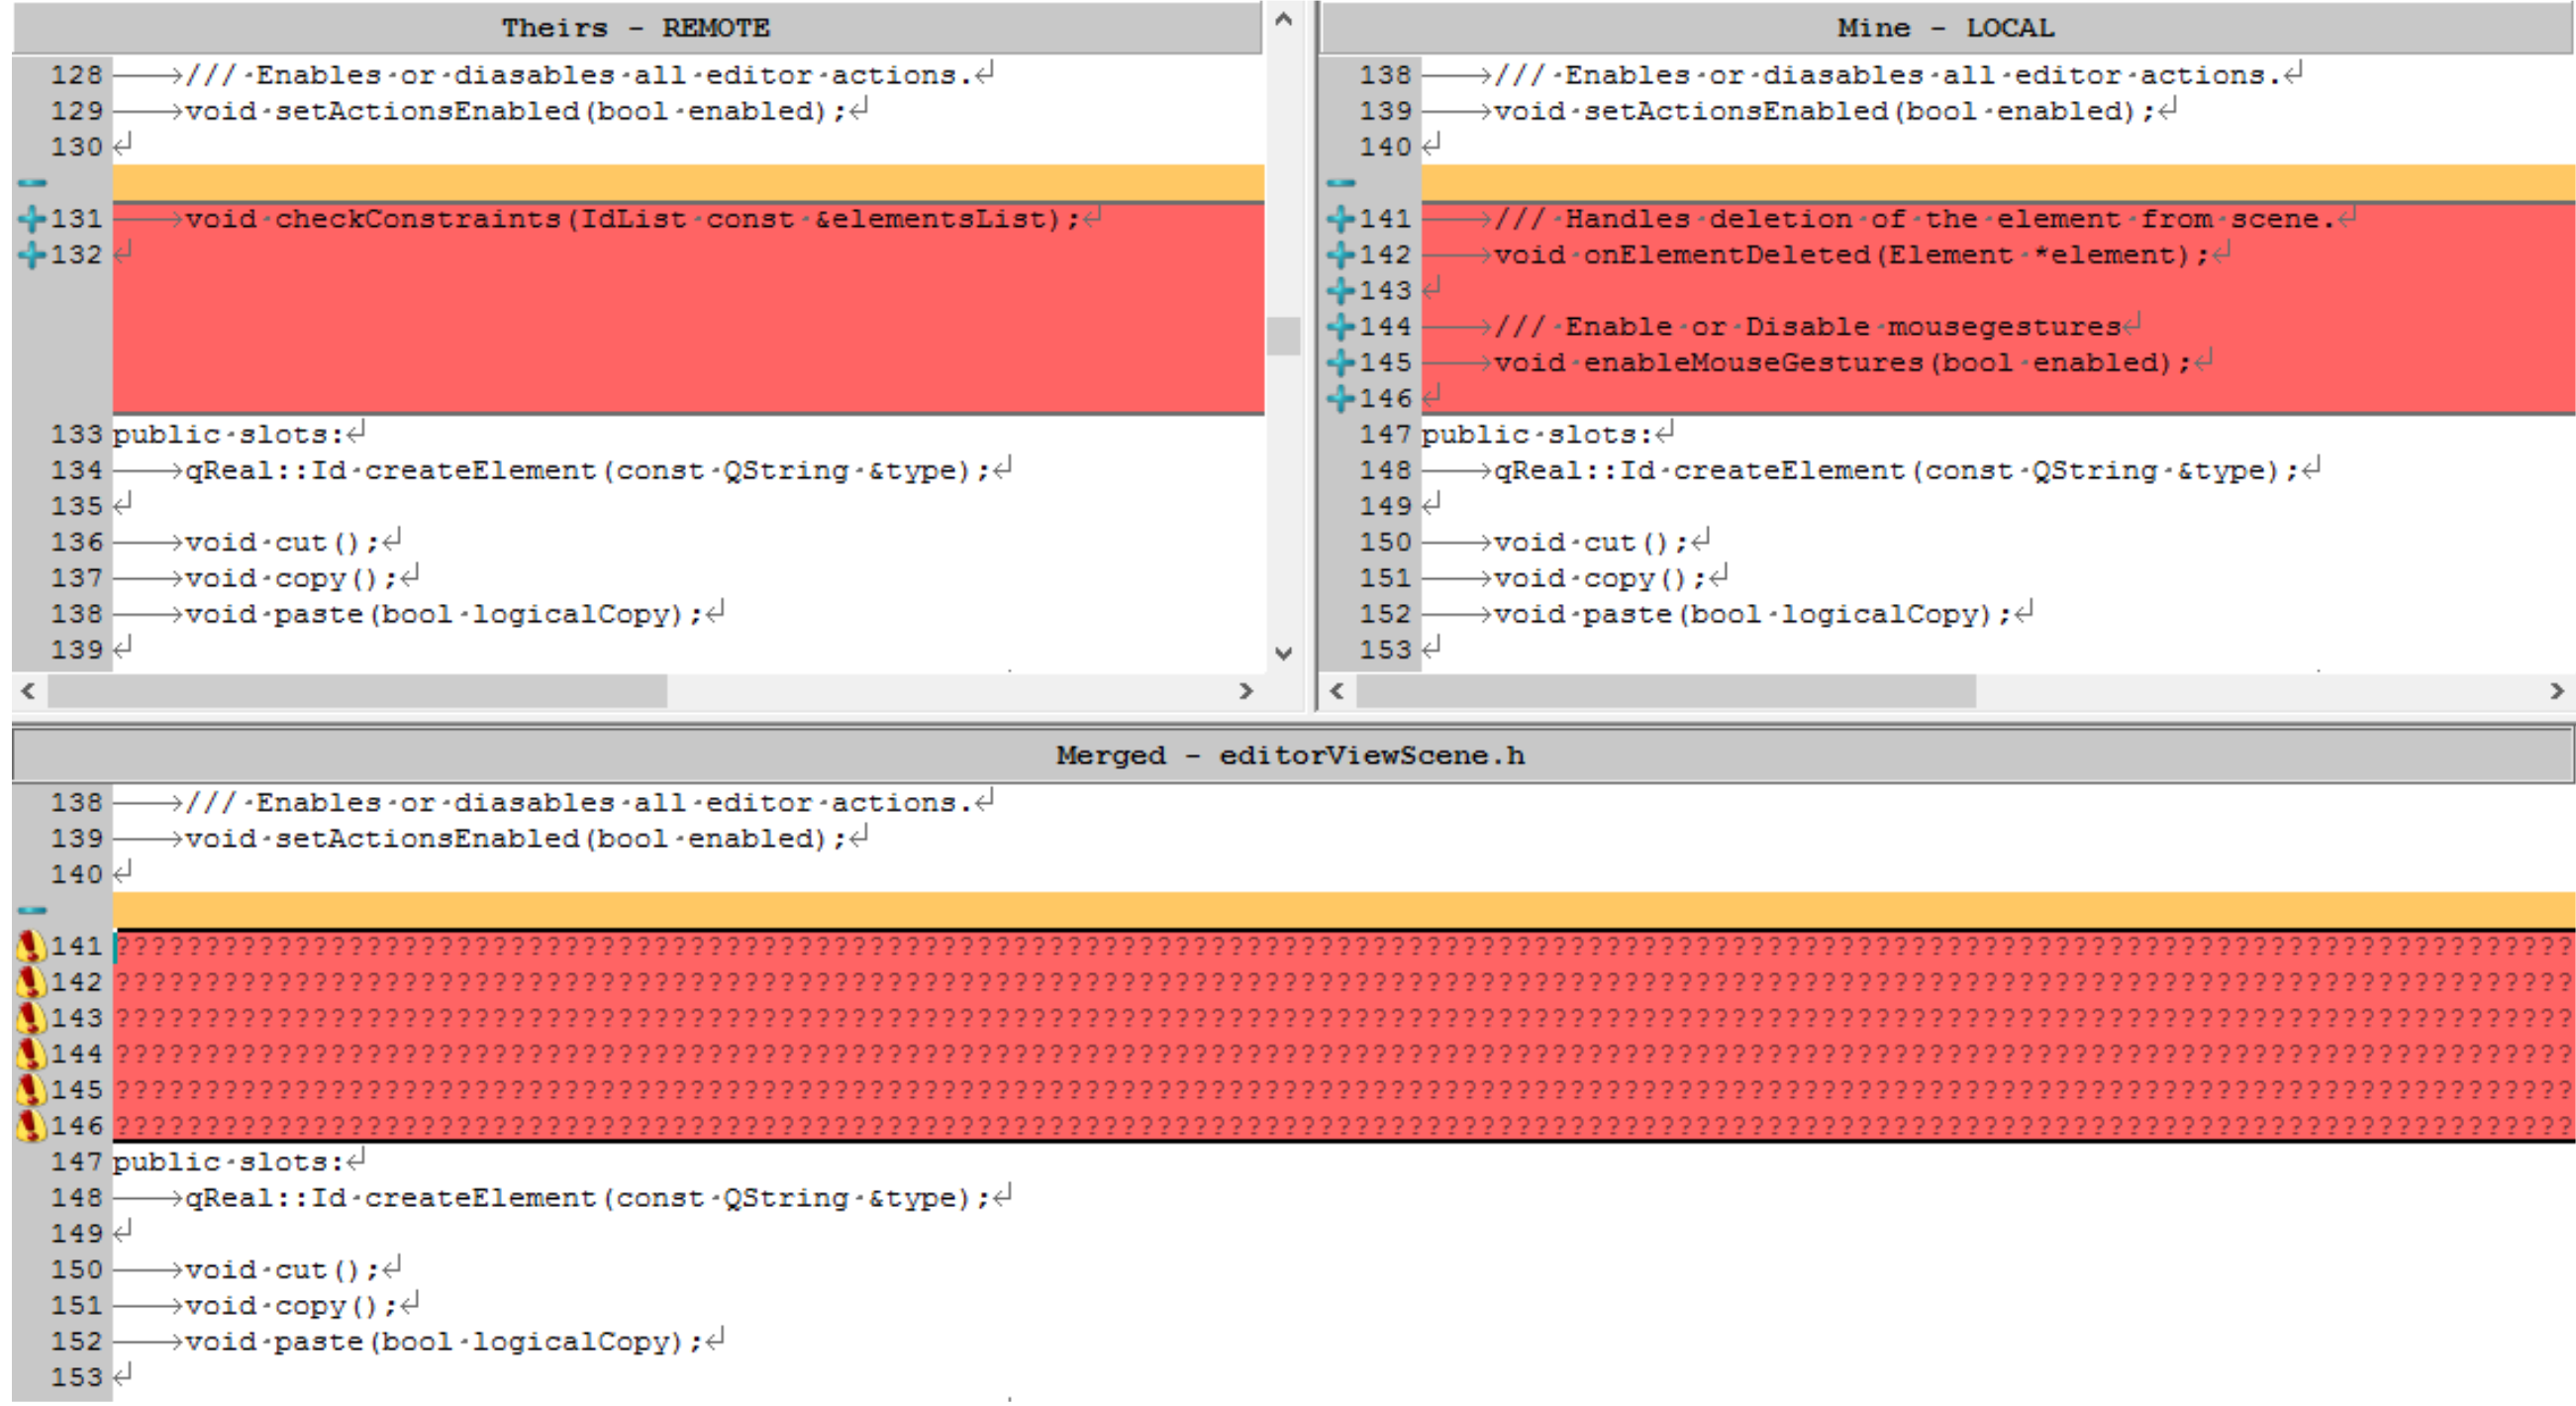
\includegraphics[width=0.95\textwidth]{conflicts.png}
\end{center}

Если вы поняли, что с конфликтами не разобраться, надо сделать 

\begin{minted}{text}
$ git merge --abort
\end{minted}

Эта команда попытается восстановить состояние рабочей копии на момент до мерджа (ей может не удасться, если после мерджа были изменения). Если вы удовлетворены процессом мерджа, надо сделать коммит, но не писать комментарий --- для мердж-коммитов комментарий сгенерится автоматически. Если вы сделали мердж-коммит, но потом начали об этом жалеть, то поможет git reset. Если откатить merge commit, то с точки зрения гита мерджа словно бы и не было.

Кстати, мердж имеет один специальный случай --- fast-forward. Это когда мы делаем мердж с веткой, которая уже содержит все наши коммиты (например, когда делаете git pull придя утром на работу и не успев ещё ничего написать). В таком случае ваша ветка просто продвигается до той, которую вы мерджите, никаких попыток посчитать диффы и найти конфликты не делается.

\subsection{git rebase}

Merge --- это не единственный и иногда даже не самый предпочтительный способ слить изменения из двух веток. Некоторые проекты активно используют команду git rebase, которая концептуально работает так:

\begin{itemize}
	\item находится общий родитель двух веток;
	\item вычисляются и сохраняются в отдельные файлы диффы, привнесённые каждым коммитом нашей ветки;
	\item наша ветка переставляется на ту ветку, на которую мы делаем rebase;
	\item все диффы применяются заново, создаются новые коммиты и добавляются в нашу ветку.
\end{itemize}

\begin{minted}{text}
$ git checkout experiment
$ git rebase master
First, rewinding head to replay your work on top of it...
Applying: added staged command
\end{minted}

\begin{center}
	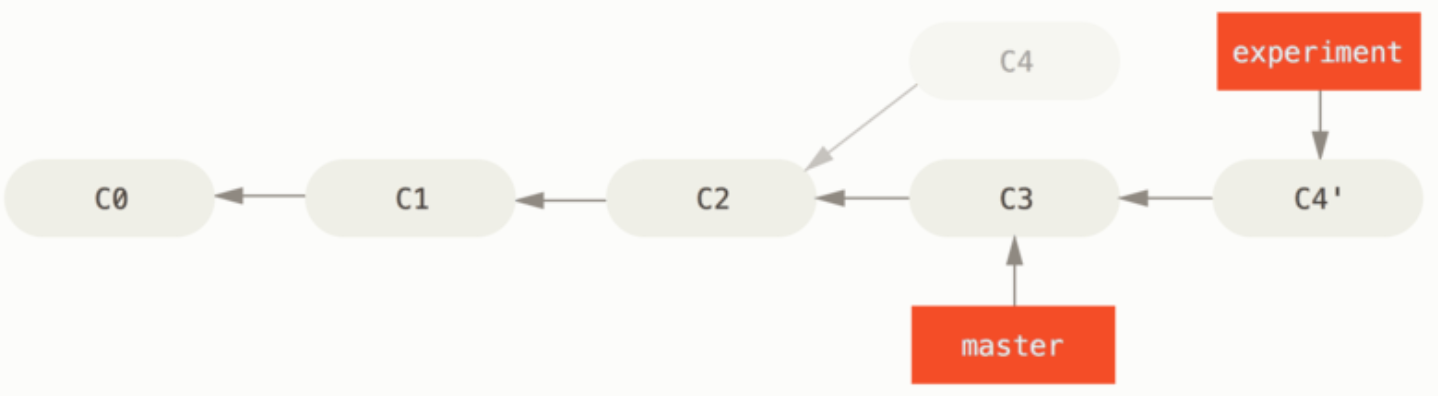
\includegraphics[width=0.8\textwidth]{rebase.png}
	\attribution{https://git-scm.com/book/ru}
\end{center}

Короче, rebase переставляет ``корень'' нашей ветки на голову той ветки, на которую мы делаем rebase. Естественно, меняя историю проекта.

Потом можно сделать обычный merge, он по определению пройдёт хорошо, потому что будет гарантированно fast-forward. Конфликты тут возможны только при применении диффов, и, что приятно в rebase, с каждым диффом будет предложено разобраться отдельно. То есть если вы давно не мерджились, merge вывалит вам один большой конфликт, rebase --- сотню маленьких и простых конфликтов.

merge против rebase --- на самом деле повод для святых войн в сообществе, потому что они делают, в общем-то, одно и то же --- сливают изменения в двух ветках. merge используют люди, которые рассматривают git как историю развития проекта и хотят знать, кто когда какую ветку отвёл и когда вмерджил. rebase используют люди, которые считают, что это не важно, важнее ``чистая'' история без тысяч веток, хаотично мерджащихся друг с другом.

В любом случае, важно помнить, что rebase создаёт новый коммит. Дату и автора rebase сохраняет, но меняется родитель, соответственно, меняется и хеш. Поэтому нельзя делать rebase уже опубликованной ветки --- если кто-то успел утянуть из неё коммиты, после rebase смерджиться будет уже невозможно. Хорошая практика во многих open-source-проектах --- перед пуллреквестом сделать rebase на текущий мастер, чтобы мэйнтейнер мог его ``чисто'' смерджить. А вот уже лежащую в репозитории ветку надо мерджить честным git merge.

\subsection{Тэги}

Ещё в Git есть тэги --- это неизменяемые указатели на коммиты. Ветки продвигаются по мере выполнения коммитов, мерджей и всего такого, тэги --- это те же ветки, но указывающие всегда на тот коммит, на который они указывали при создании (на самом деле, можно удалить тэг и создать такой же на другой коммит, но ваши коллеги не одобрят). Тэги используются, чтобы давать человеческие имена разным интересным коммитам, например, коммиту, из которого был собран релиз такой-то версии.

Тэги в Git бывают двух сортов --- легковесные и аннотированные. 

\begin{itemize}
	\item Легковесный тэг:
		\begin{minted}{text}
git update-ref refs/tags/v1.0 cac0cab538b970a37ea1e769cbbde608743bc96d
		\end{minted}
		Или просто git tag. Это не более чем просто создание ссылки на коммит.
	\item Аннотированный тэг:
		\begin{minted}{text}
$ git tag -a v1.1 -m 'test tag'
		\end{minted}
		--- это отдельный объект (то есть отдельный файл в репозитории), хранящий в себе аннотацию тэга (то есть его имя), комментарий, автора и дату создания. И на него же указывает ссылка с человеческим именем (в данном случае, v1.1). Аннотированные тэги обычно полезнее.
\end{itemize}

\subsection{Внутреннее хранение данных в Git}

Пока что получалось, что все версии всех файлов в Git хранятся целиком, как они есть. Все они всегда сжимаются zlib, но в целом, если создать репозиторий, добавлять туда файлы, коммитить и т.д., все версии всех файлов будут в нём целиком. Это очень печально, потому что активно развивающийся проект может иметь десятки тысяч коммитов, каждый из которых затрагивает десятки или сотни файлов. И потом, есть же дельта-компрессия, которая всю жизнь использовалась в Subversion и других системах контроля версий. Поэтому в Git есть понятие .pack-файла. 

Pack-файл --- это собранные в один файл файлы из репозитория, упакованные как раз с помощью дельта-компрессии. Git при упаковке пытается найти все похожие файлы, один из них он сохраняет полностью, остальные ссылаются на какой-то другой файл и хранят дельту. Таким образом, при распаковке, если мы хотим получить конкретный файл (например, версию, относящуюся к такому-то коммиту), мы можем пробежаться по цепочке ссылок в .pack-файле и восстановить текущую версию из исходной, последовательно применив дельты (в точности как в Subversion). Отличие от Subversion состоит в том, что Git делает дельта-компрессию с большой неохотой, только иногда (причём, без вашего ведома) и оставляет снапшоты полных файлов раз в сколько-то коммитов, чтобы не применять дельты с самого-самого начала, а только от ближайшего полного снапшота. В общем-то, понятно, почему --- место на жёстком диске нынче дешёвое, текстовые файлы всё равно весят мало, так что смысла старательно сжимать репозиторий дельта-компрессией никакого нет. А хочется, чтобы частые команды работали очень быстро. Вполне возможно, что для большинства ваших проектов Pack-файлы не будут созданы вообще никогда.

Помимо файла .pack есть файл .idx --- индекс Pack-файла. В нём хранится отображение хешей файлов на адреса внутри Pack-файла, чтобы можно было быстро найти нужный файл:

\begin{center}
	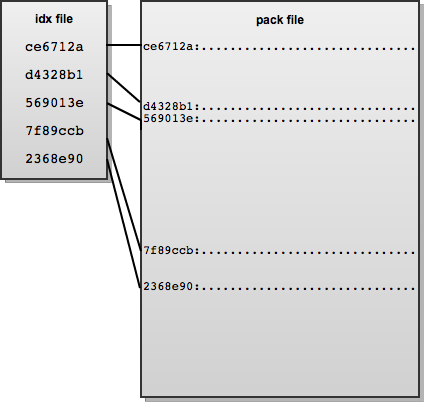
\includegraphics[width=0.4\textwidth]{gitPackFiles.png}
\end{center}

\section{Хорошие практики}

Вот некоторые общеупотребимые практики при работе с системами контроля версий вообще и с Git в частности:

\begin{itemize}
	\item Коммитим только исходные тексты, конфиги, картинки и т.п. Следует избегать исполнимых файлов или слишком больших нетекстовых файлов, потому что для них дельту не посчитать.
	\item Если что-то может быть автоматически сгенерировано по тому, что уже есть в репозитории, это НЕ коммитим. Ибо незачем, правильнее настроить автоматическую сборку так, чтобы это появлялось само у пользователя на машине.
	\item Всегда и обязательно пишем адекватные комментарии к коммитам. Обычно комментарий --- это одно-два полных осмысленных предложения, описывающих, что же было добавлено в проект предлагаемыми изменениями. Причём, не какие файлы (это и так видно в логе), а что по сути --- фичи, фиксы багов (обязательно со ссылкой на нужный баг) и т.д. Комментарии типа ``fix'' будут жестоко караться в домашке.
	\item Коммитим как можно чаще. Сделали что-то осмысленное --- коммит. Единственное требование --- чтобы закоммиченный код компилировался.
	\item Коммит не должен содержать в себе файлы, не относящиеся к изменениям. Поэтому нежелательно пользоваться ключом -a к git commit, очень желательно иметь правильный .gitignore и обязательно перед коммитом проверять, что же вы коммитите (git status как минимум, git diff желательно). То же касается пуллреквестов --- никогда не ленитесь смотреть diff.
	\item Коммит не должен добавлять/убирать пустые строки, менять пробелы на табы и т.д., если это не суть коммита. Такого рода изменения надо делать отдельными коммитами, иначе изменений по существу не будет видно в диффе.
	\item Стиль исходного кода и отступов должен совпадать с текстом вокруг. Особенно это касается больших проектов, надо обязательно либо прочитать местный стайлгайд, либо посмотреть на соседний код. Со своими порядками в чужой монастырь не ходят, сколь бы разумными вам ни казались эти порядки.
\end{itemize}

Ещё есть практика использования веток в репозитории, которая называется Git Flow и рекомендуется к использованию GitHub. Про неё знают некоторые инструменты и умеют явно поддерживать. Суть её в правильном использовании веток и следовании некоторым соглашениям:

\begin{itemize}
	\item ветка master используется для хранения стабильных релизов, чтобы если кто-то сделает git clone, у него всё без проблем собралось и запустилось;
	\item основная разработка ведётся в ветке develop, в ней всегда самый свежий код и в неё мерджатся все изменения;
	\item собственно изменения (такие как реализация новой фичи или багфикс) делаются в отдельных ветках, по одной ветке для каждого изменения. Ветки отводятся от develop в начале разработки и мерджатся в develop, когда фича или багфикс закончены. Обычно в каждой такой ветке ведёт работу один член команды, и обычно время жизни таких веток невелико --- в идеале измеряется часами.
	\item Как только код в develop готов к релизу, отводится релизная ветка. В релизную ветку мерджатся только багфиксы к релизу, а разработка в develop продолжает жить своей жизнью. Фиксы из релизной ветки мерджатся обратно в develop.
	\item Когда продукт в релизной ветке уже удовлетворительного состояния, он мерджится в мастер и объявляется релизом. В мастере создаётся тэг с номером релиза.
	\item Если в ходе эксплуатации уже зарелизенной версии выявляются критические баги, от мастера отводится ветка для хотфиксов, баги правятся в ней и вновь мерджатся в мастер (и в develop). Так появляется новый багфикс-релиз, со своим тэгом.
\end{itemize}

Вот так это примерно выглядит:

\begin{center}
	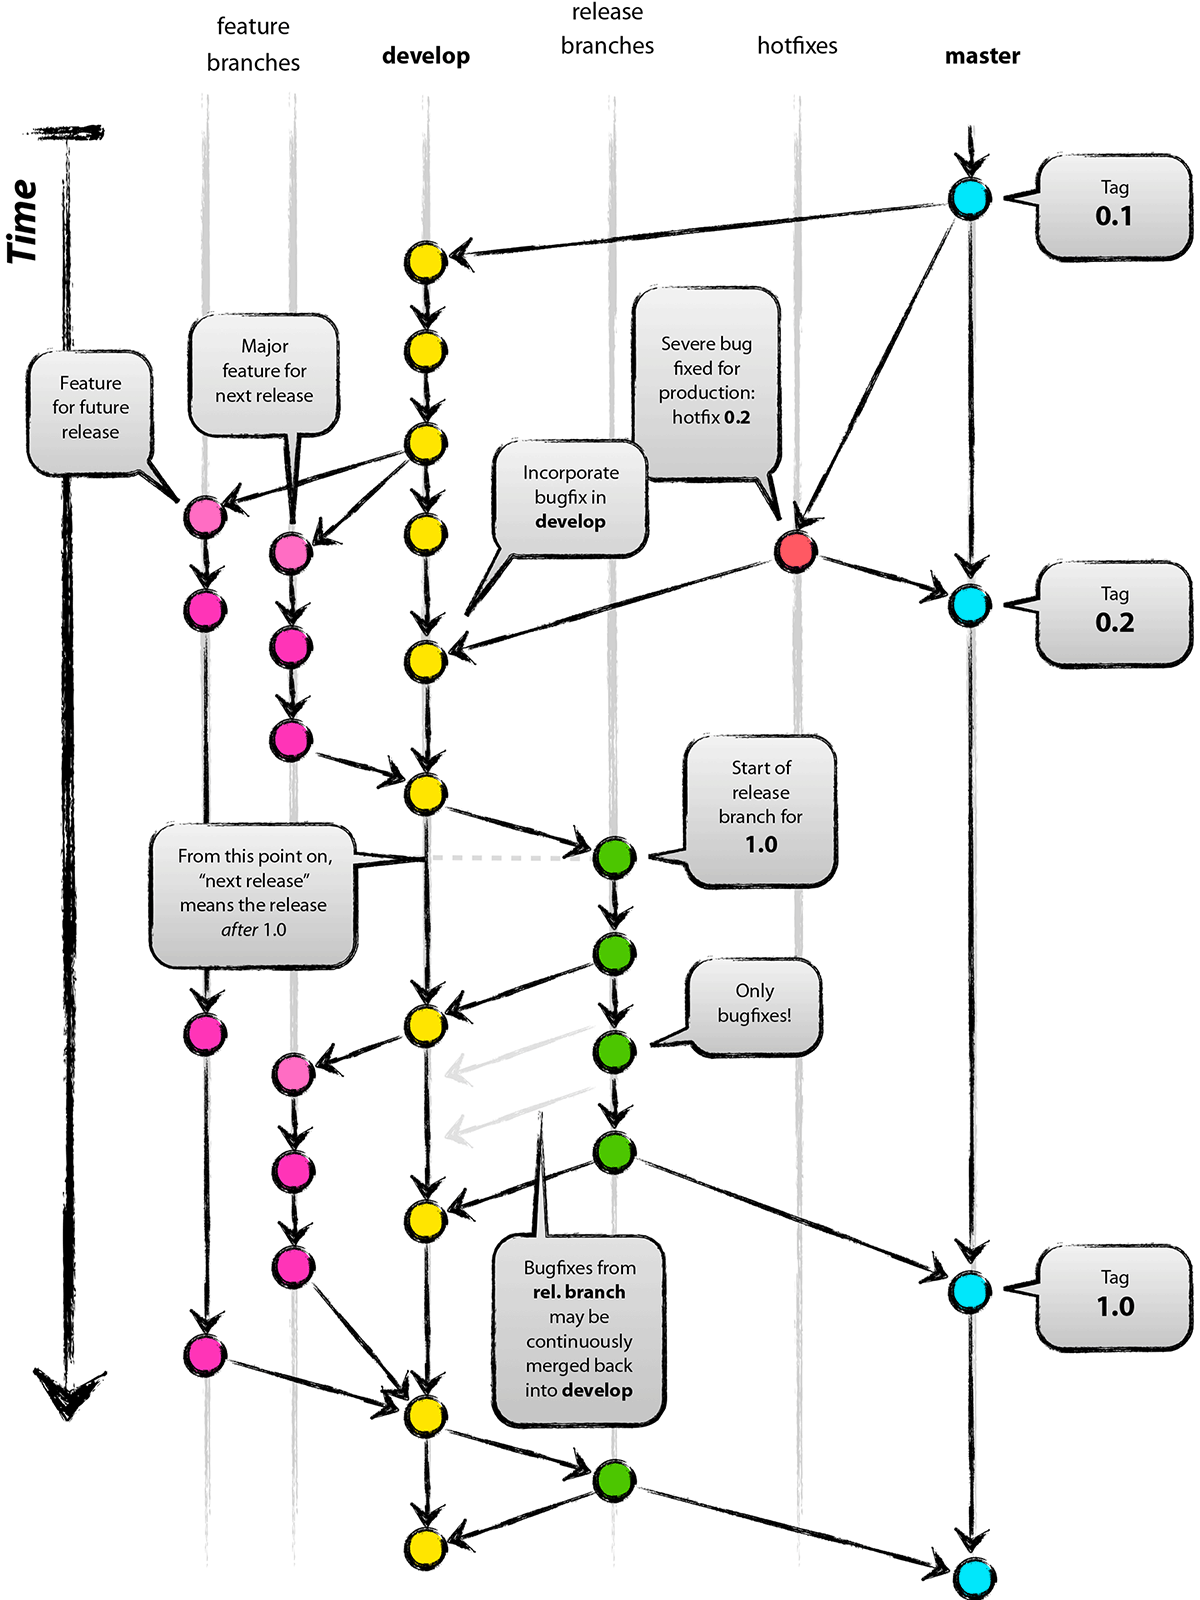
\includegraphics[width=0.7\textwidth]{gitFlow.png}
	\attribution{https://nvie.com/posts/a-successful-git-branching-model/}
\end{center}

Мы такой же модели придерживаемся в домашках, задача --- это фича, master --- ветка, где стабильный уже прошедший ревью код.

\section{Ещё полезные команды}

Ещё несколько полезных штук, которые не очень известны, поэтому о них часто даже не догадываются:

\begin{itemize}
	\item \verb|git add -p| --- интерактивное добавление изменений к коммиту, позволяет коммитить только часть файла;
	\item \verb|git commit --amend| --- исправить последний коммит;
	\begin{itemize}
		\item \verb|git commit --amend -m "an updated commit message"|.
		\item Применять \textbf{только до} git push. Изменение уже опубликованной истории коммитов может иметь ужасные последствия, как водится.
	\end{itemize}
	\item \verb|git reset --hard| --- откатить все изменения в рабочей копии до последнего коммита. Это не то чтобы малоизвестная команда, но очень полезна, особенно если вы всё испортили. Обязательно проверяйте git status, что не откатите лишнего.
	\item \verb|git reset --hard <хеш коммита>| --- откатить все изменения в текущей ветке до указанного коммита, забыть все коммиты, что были после (и случайно грохнуть всю домашку перед зачётом). В качестве хеша коммита может быть и ссылка, так что у этой команды есть одна часто применяемая форма: \verb|git reset --hard origin/master| --- откатиться до состояния, в котором находится код в удалённом репозитории. Так можно вылечить большинство проблем с тем, что вы что-то сделали не так и теперь в рабочей копии всё плохо.
	\item Все команды, которые могут испортить историю, делаются с ключом --force (или -f). Например, как откатить ветку до нужного коммита и выложить на гитхаб:
		\begin{minted}{text}
git reset --hard <хеш нужного коммита>
git push -f origin <имя ветки>
		\end{minted}
		Без ключа -f гит резонно скажет, что в удалённом репозитории версия посвежее, поэтому ничего делать он не будет. Опцию -f надо использовать очень-очень осторожно, потому что ваш репозиторий уже мог кто-то склонить, тогда будут альтернативные исторические линии, которые нельзя будет смерджить друг с другом. И так можно реально потерять работу. Зато это помогает от неудачных мерджей, неправильно отведённых веток и т.д.
	\item На крайний случай рекомендую погуглить про git cherry-pick. Это команда, которая делает из коммита дифф и применяет его туда, куда вы скажете. То есть можно выбрать любой коммит из истории одной ветки и применить его поверх другой. При этом создаётся новый коммит и старый не удаляется (так что эти две ветки уже не получится смерджить), но это может быть полезным инструментом в запущенных случаях. git rebase --onto может помочь, если таких коммитов много, но про него тоже погугите самостоятельно (это не то чтобы часто используется и не то чтобы хороший стиль).
\end{itemize}

\section{.gitignore}

Файл .gitignore нужен для того, чтобы указать git, какие файлы должны игнорироваться системой контроля версий вообще --- то есть не показываться в git status, в git diff, не предлагаться добавиться в коммиты и т.д. Очень полезный инструмент, чтобы не коммитить случайно то, что не должно быть закоммичено. Кстати, уже закомиченные файлы остаются в репозитории, если их прописать в .gitignore, поэтому .gitignore очень желательно писать заранее. 

Бывает глобальный .gitignore (но не очень понятно, зачем он нужен), бывает локальный для репозитория, который выкладывается в гит вместе с другими файлами. Вообще, .gitignore может быть хоть для каждой папки в репозитории свой, но обычно этого не нужно и его кладут прямо в корень репозитория.

Содержимое файла --- это набор Glob-шаблонов и комментариев. Комментарии начинаются с \# (как в sh). Синтаксис glob-шаблонов такой:

\begin{itemize}
	\item \mintinline{text}|*| --- 0 или более символов;
	\item \mintinline{text}|?| --- один символ;
	\item \mintinline{text}|[abc]| --- любой символ из указанных в скобках;
	\item \mintinline{text}|[0-9]| --- любой символ из интервала;
	\item Шаблоны, начинающиеся со /, сопоставляются только в корне репозитория;
	\item Шаблоны, заканчивающиеся на /, сопоставляются только с каталогами;
	\item \mintinline{text}|**| в теле шаблона сопоставляется с вложенными каталогами;
	\item Шаблоны, начинающиеся на ! --- отрицание шаблона, записанного за !.
\end{itemize}

Вот небольшой пример из документации:

\begin{minted}{bash}
# не обрабатывать файлы, имя которых заканчивается на .a
*.a
# НО отслеживать файл lib.a, несмотря на то, что мы игнорируем все .a файлы 
!lib.a
# игнорировать только файл TODO, находящийся в корневом каталоге
/TODO
# игнорировать все файлы в каталоге build/
build/
# игнорировать doc/notes.txt, но не doc/server/arch.txt
doc/*.txt
# игнорировать все .txt файлы в каталоге doc/
doc/**/*.txt
\end{minted}

На самом деле, всё написано за нас, и GitHub даже поддерживает репозиторий с популярными файлами .gitignore, которые можно копипастить себе и по-разному комбинировать: \url{https://github.com/github/gitignore}

\end{document}
